\section{Methodology}

\subsection{Project Deliverables}

This research project delivers the following outcomes:

\begin{itemize}
    \item A literature review focussed on data quality monitoring in smart cities.
    \item A taxonomy of data quality dimensions for object-detecting wireless sensor networks.
    \item A machine learning pipeline for automated data quality monitoring of pedestrian data streams.
    \item A pathway to a real-time monitoring system for detecting data quality issues in smart city data streams
    \item A dashboard for visualising data quality issues.
\end{itemize}

The key scientific discoveries that this research project seeks to make are:

\begin{itemize}
    \item Understanding how and why data quality issues occur in smart city data streams.
    \item Identifying the key data quality dimensions that are important for smart city data streams.
    \item Finding the limits of sparsity and noise in data used for predictive modelling (what is the minimum quality of data required for accurate predictions?).
\end{itemize}

\subsection{Overview}

This methodology section outlines the research design and implementation of the project. The Research Design Section \ref{research_design} focusses on explaining the rationale behind the choices made in the experiment design. The Implementation Section \ref{implementation} gives a brief overview as to how these design decisions have been implemented. A detailed description of the implementation, including a guide explaining how you can run your own experiment using the library, is provided in the package documentation which can be found \href{https://carrowmw.github.io/phd-project/pipeline_module/overview/}{here}.

\subsection{Research Design} \label{research_design}

The research design is structured into the following stages:

\begin{enumerate}
    \item Data Collection
    \item Data Preprocessing
    \item Feature Engineering
    \item Data Loading
    \item Model Training
    \item Model Evaluation
\end{enumerate}

\subsubsection{Data Collection}

The Newcastle Urban Observatory is one of the worlds largest open urban data collection projects. The data collected includes pedestrian counts, air quality, weather, and traffic data. The high velocity data streams are available in near real-time for a wide range of sensor types, including object-detecting wireless sensors - which are the focus of this research project. The depth and breadth of the data collected by the urban observatory make it an ideal case study for investigating for understanding the causes of data quality issues and the effect of issues on predictive modelling. The map in Figure \ref{fig:map_of_sensors} shows the distribution of pedestrian sensors across the city of Newcastle.

\begin{figure}[H]
    \centering
    \adjustbox{width=0.90\linewidth, keepaspectratio}{%
        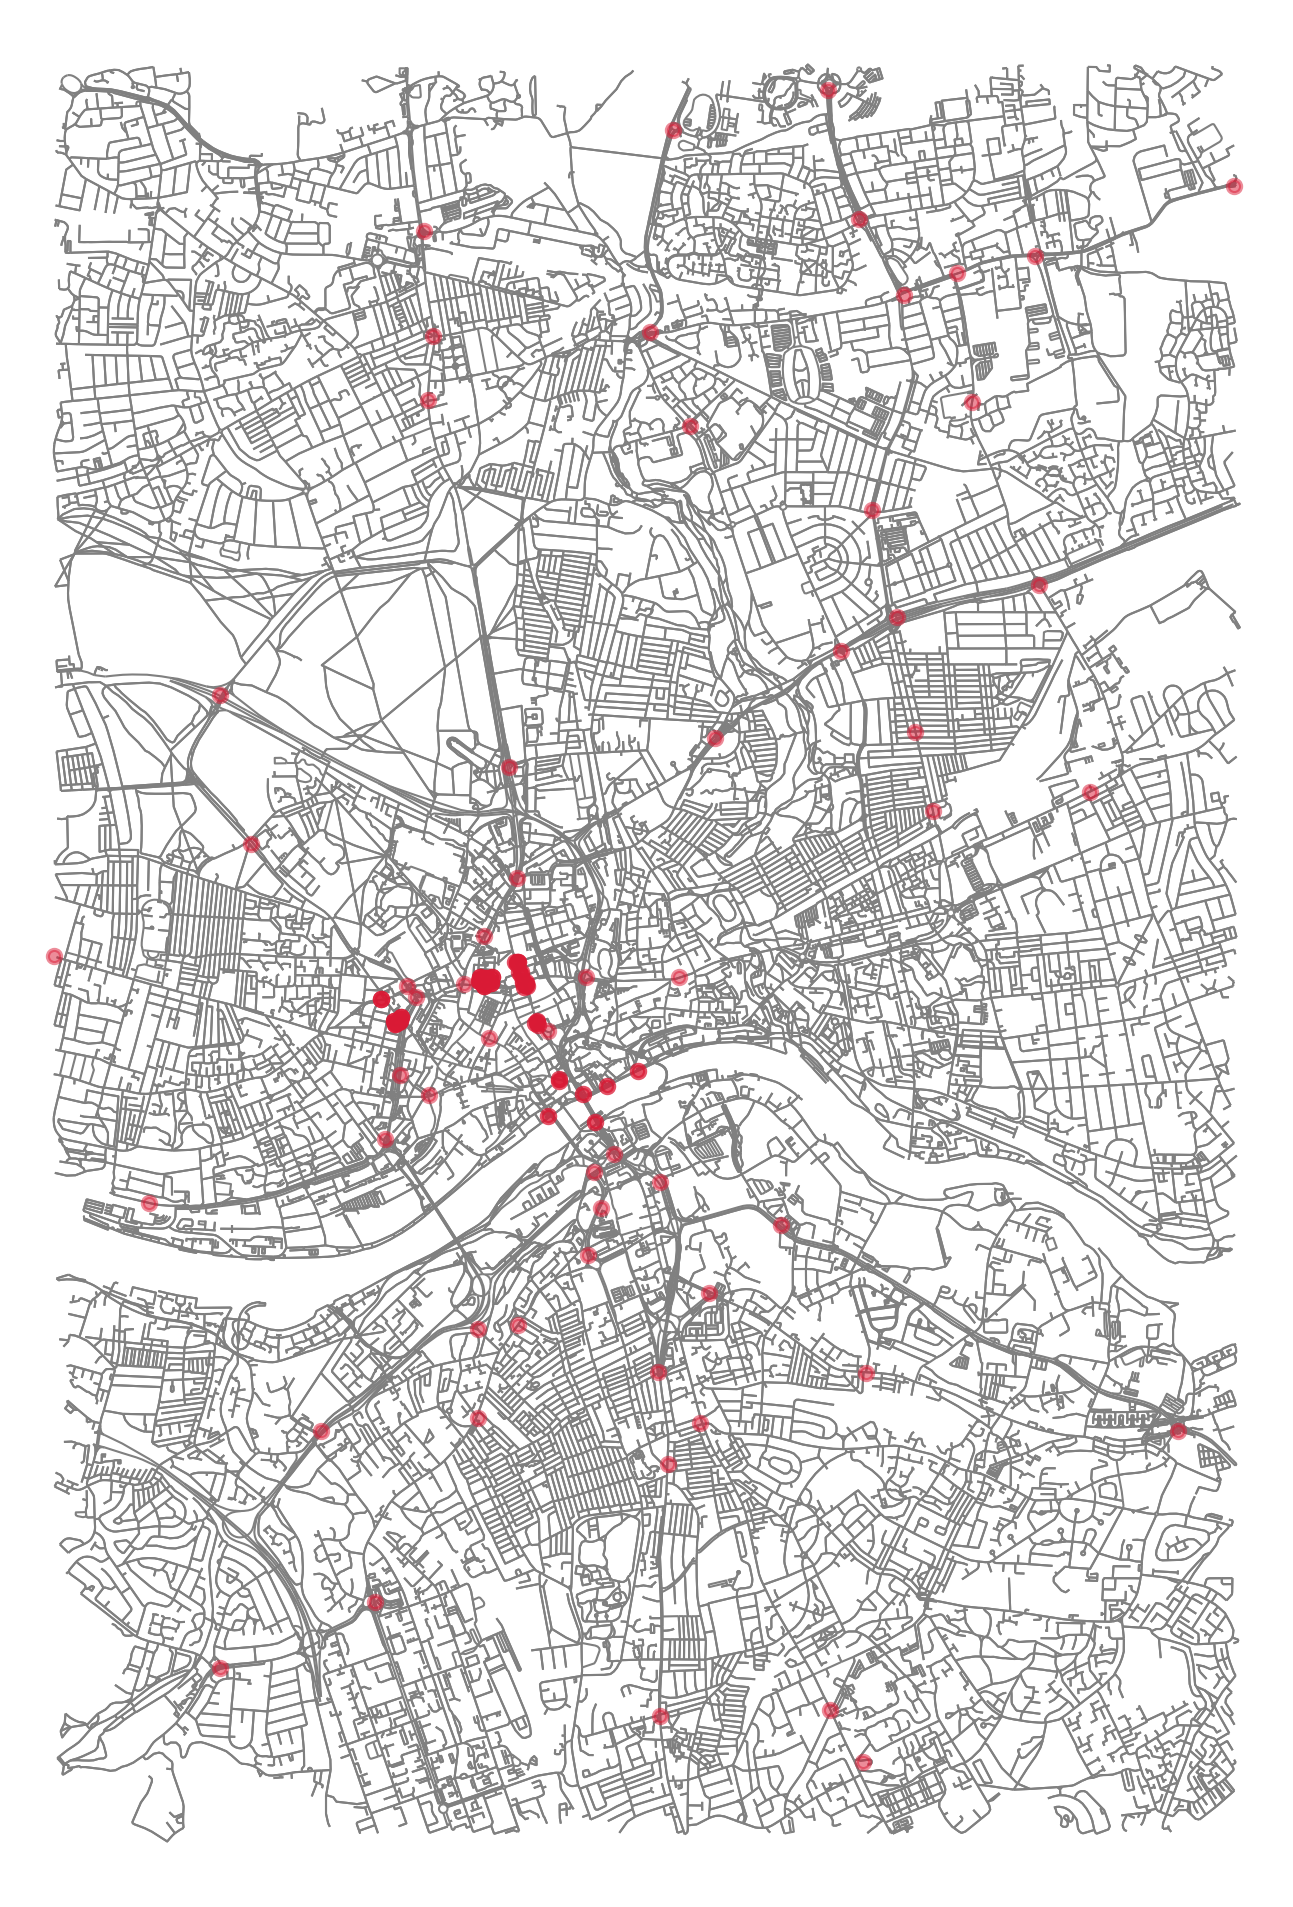
\includegraphics{figures/methodology/map_of_sensors.png}%
    }
    \caption{Distribution of sensors in the urban observatory}
    \label{fig:map_of_sensors}
\end{figure}

The data from the pedestrian sensors is collected at 15-minute intervals and each record contains the number of pedestrians detected within a scene over that time period. Figure \ref{fig:preprocessed_data_example_timeseries} shows an example of the raw data from a sensor over a period of 18 days in February 2023. The y-axis shows the number of pedestrians recorded by the sensor over a 15-minute period. The x-axis is the timestamp of the recording. The full extent of the data for the same sensor is shown in Figure \ref{fig:preprocessed_data_example_timeseries_full}. Both Figure \ref{fig:preprocessed_data_example_timeseries} and Figure \ref{fig:preprocessed_data_example_timeseries_full} show that there are data quality issues. Figure \ref{fig:preprocessed_data_example_timeseries} shows regular missing data points during the night (when there are no pedestrians) and Figure \ref{fig:preprocessed_data_example_timeseries_full} shows that there are some extended periods of data sparsity.

\begin{figure}[H]
    \centering
    \adjustbox{width=0.90\linewidth, keepaspectratio}{%
        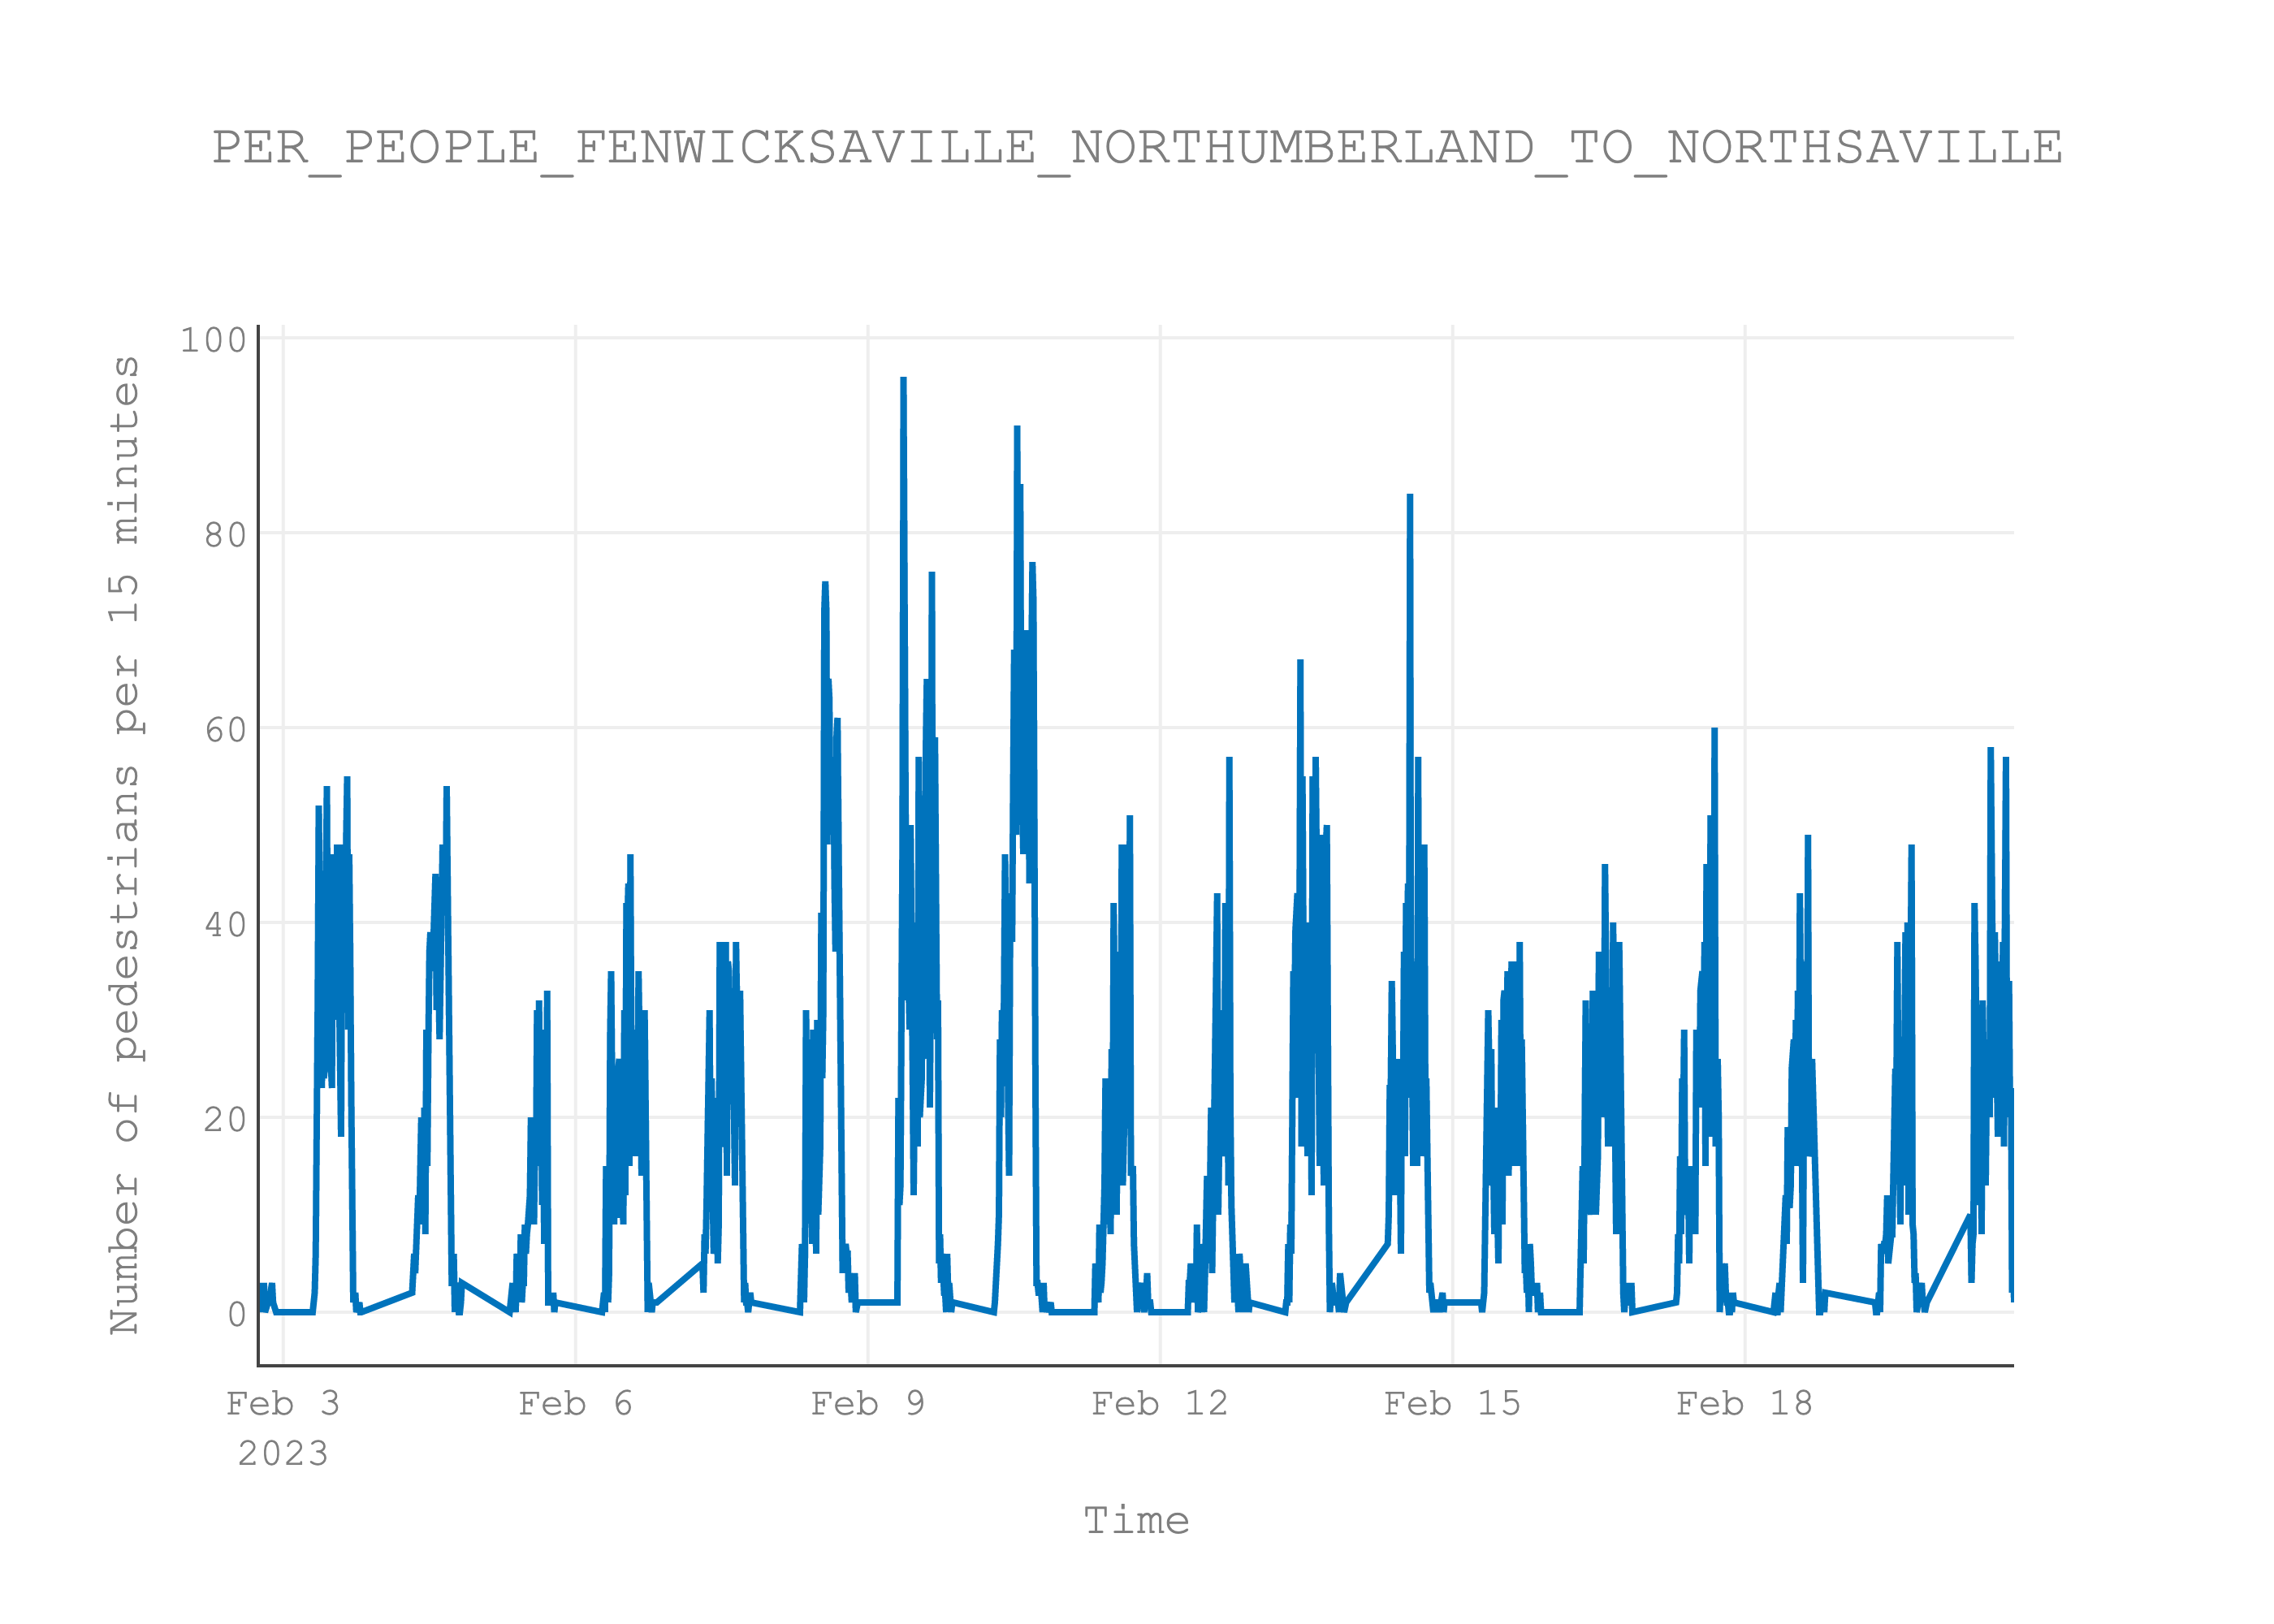
\includegraphics{figures/methodology/preprocessed_data_example_timeseries.png}%
    }
    \caption{Example of preprocessed data from a sensor}
    \label{fig:preprocessed_data_example_timeseries}
\end{figure}

\begin{figure}[H]
    \centering
    \adjustbox{width=0.90\linewidth, keepaspectratio}{%
        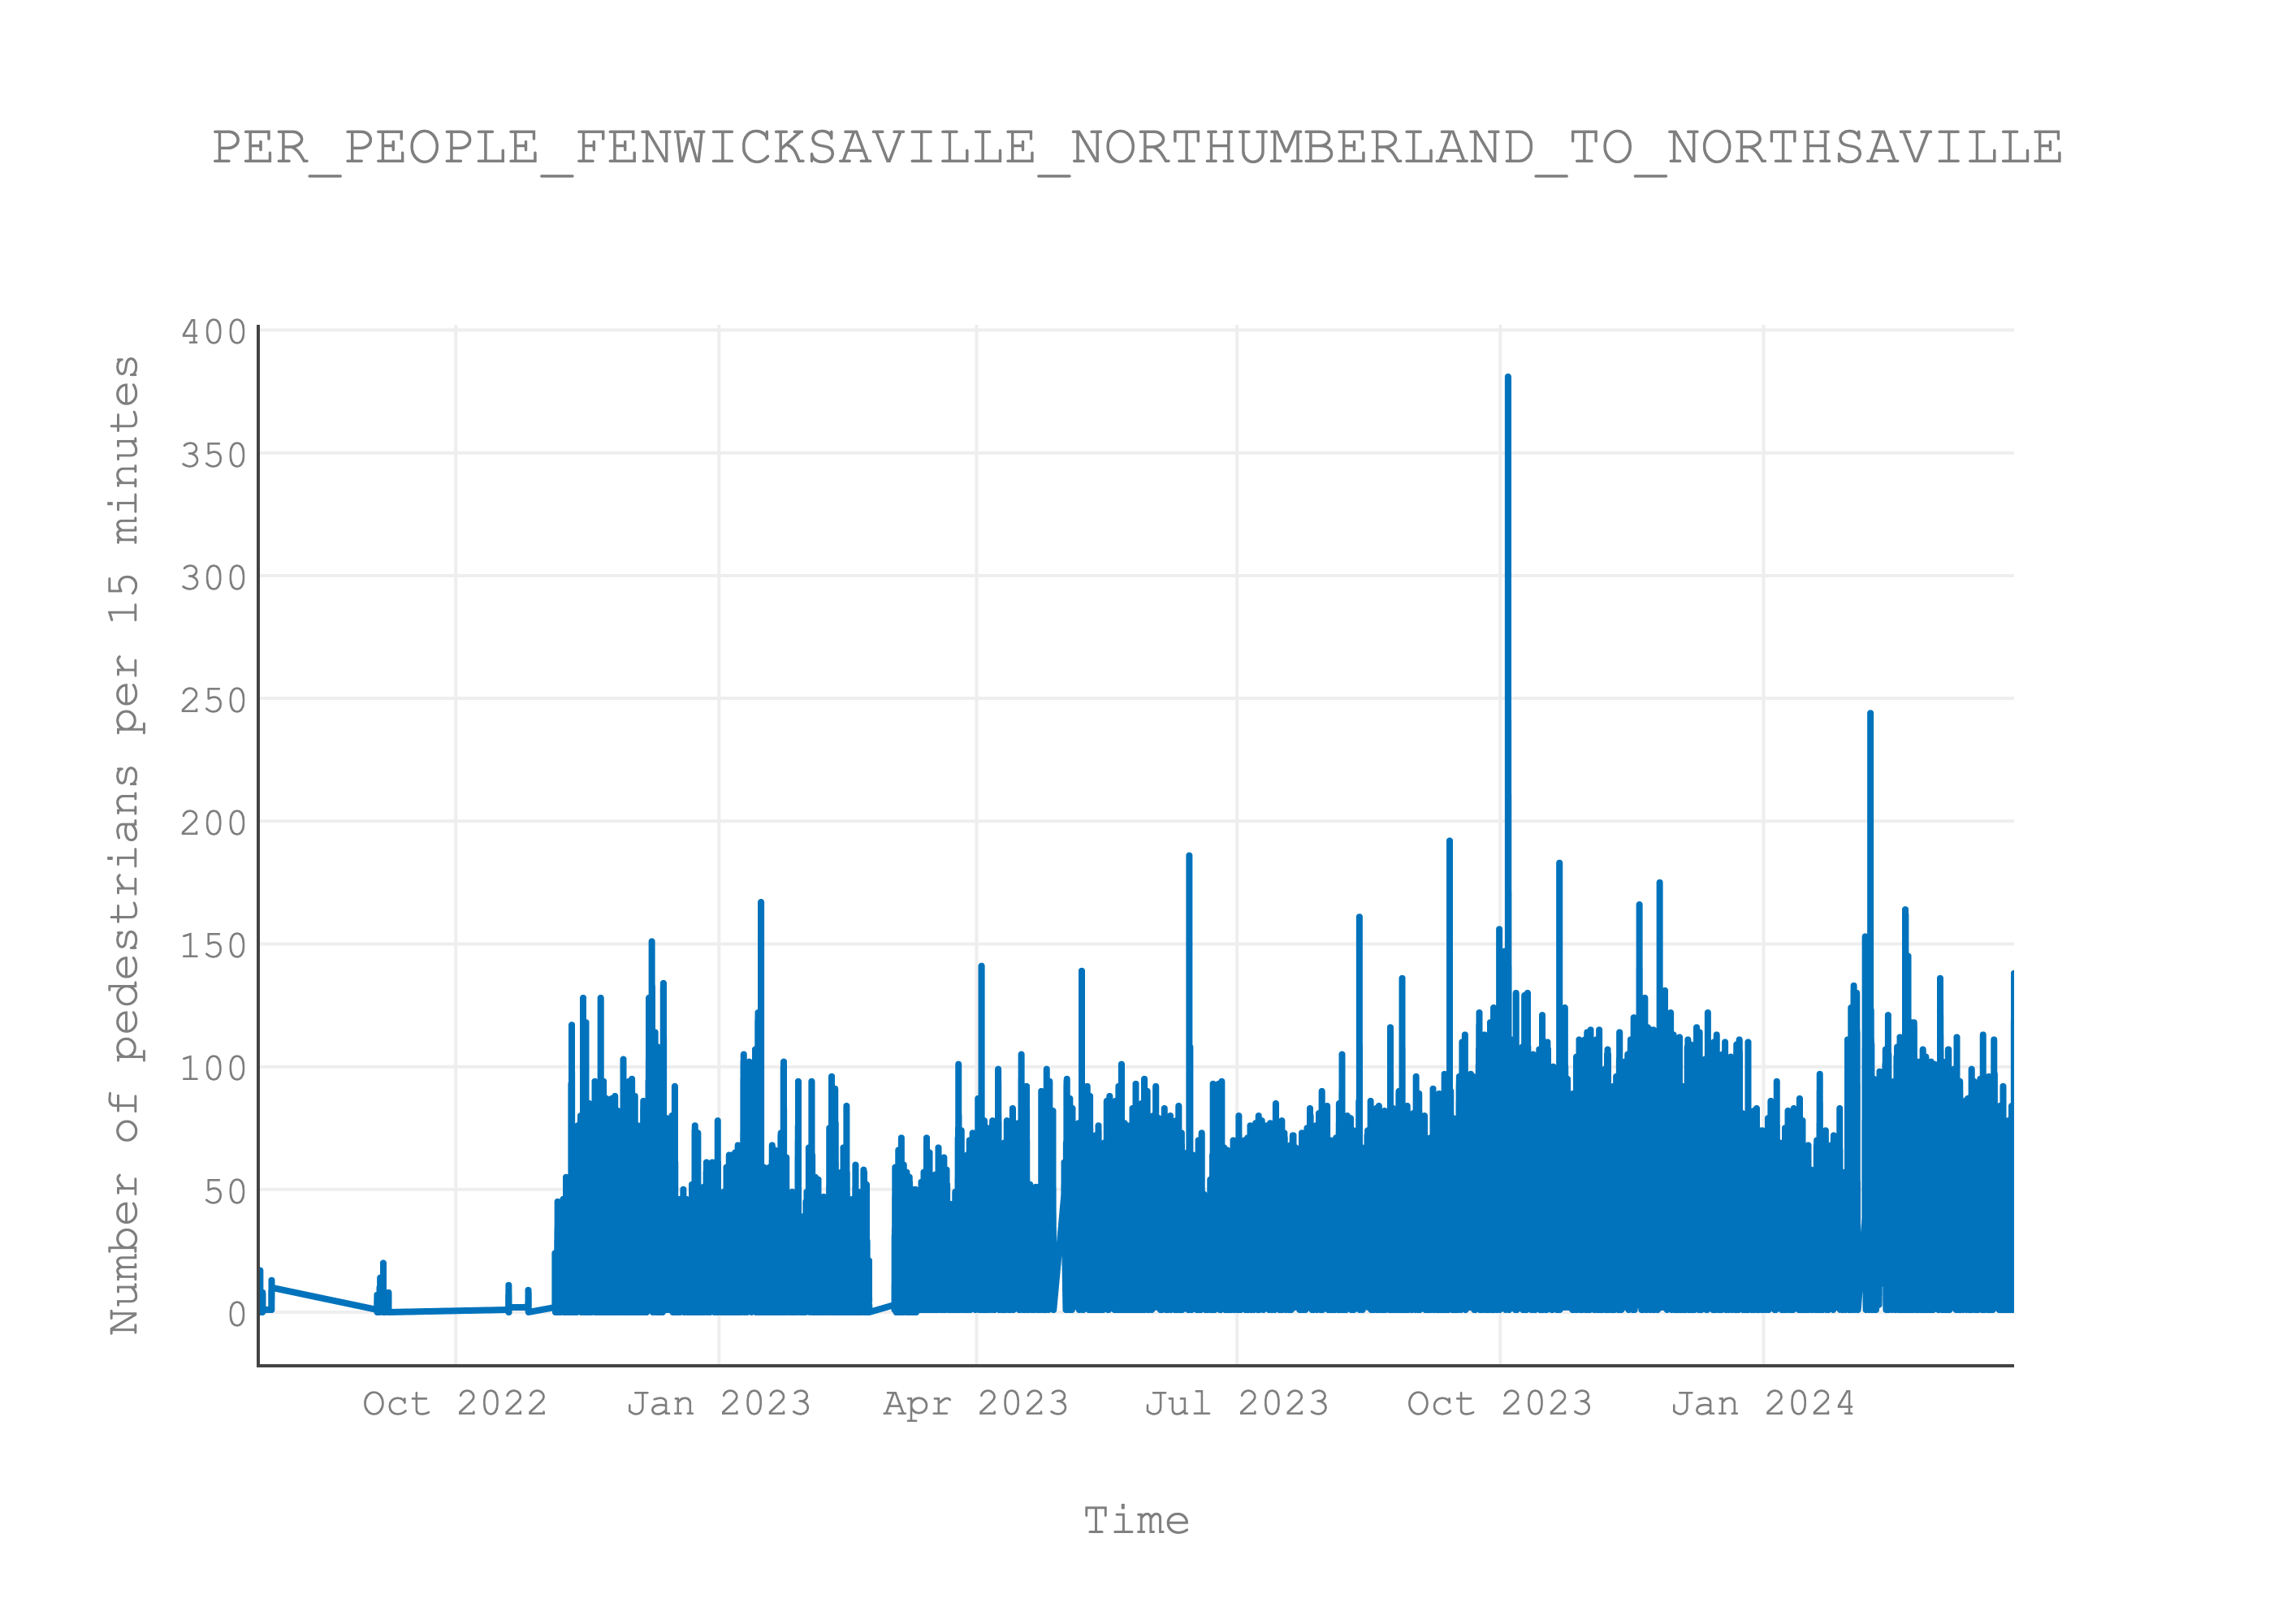
\includegraphics{figures/methodology/preprocessed_data_example_timeseries_full.png}%
    }
    \caption{Example of preprocessed data from a sensor - 2-year extent}
    \label{fig:preprocessed_data_example_timeseries_full}
\end{figure}

The data quality issues in the urban observatory data can be summarised as follows:

\begin{itemize}
    \item Missing data points - these are caused by sensor failures, networks issues, or sensor design issues (some of the sensors do not transmit a reading if there are no pedestrians detected).
    \item Erroneous data points - these result from a range of issues such as sensor calibration issues, network issues, or environmental factors (e.g. a sensor may be blocked by a parked lorry). Due to the nature of the data (raw sensor footage is unavailable due to data protection guidelines), it is difficult to determine the cause of the erroneous data points, or if they are indeed erroneous. This presents an interesting challenge for the research project.
\end{itemize}

To more clearly indicate the extent of the missing data points, Figure \ref{fig:records_per_day_example} shows the number of records recorded per day for the same sensor. The plot shows that there are many missing records over the 2-year period. Ideally there should be 96 records per day (4 records per hour for 24 hours). The plot shows that there are approximately zero days where all 96 records are present. It is also evident from Figure \ref{fig:records_per_day_example} that there are a few days where no records are present at all.

\begin{figure}[H]
    \centering
    \adjustbox{width=0.90\linewidth, keepaspectratio}{%
        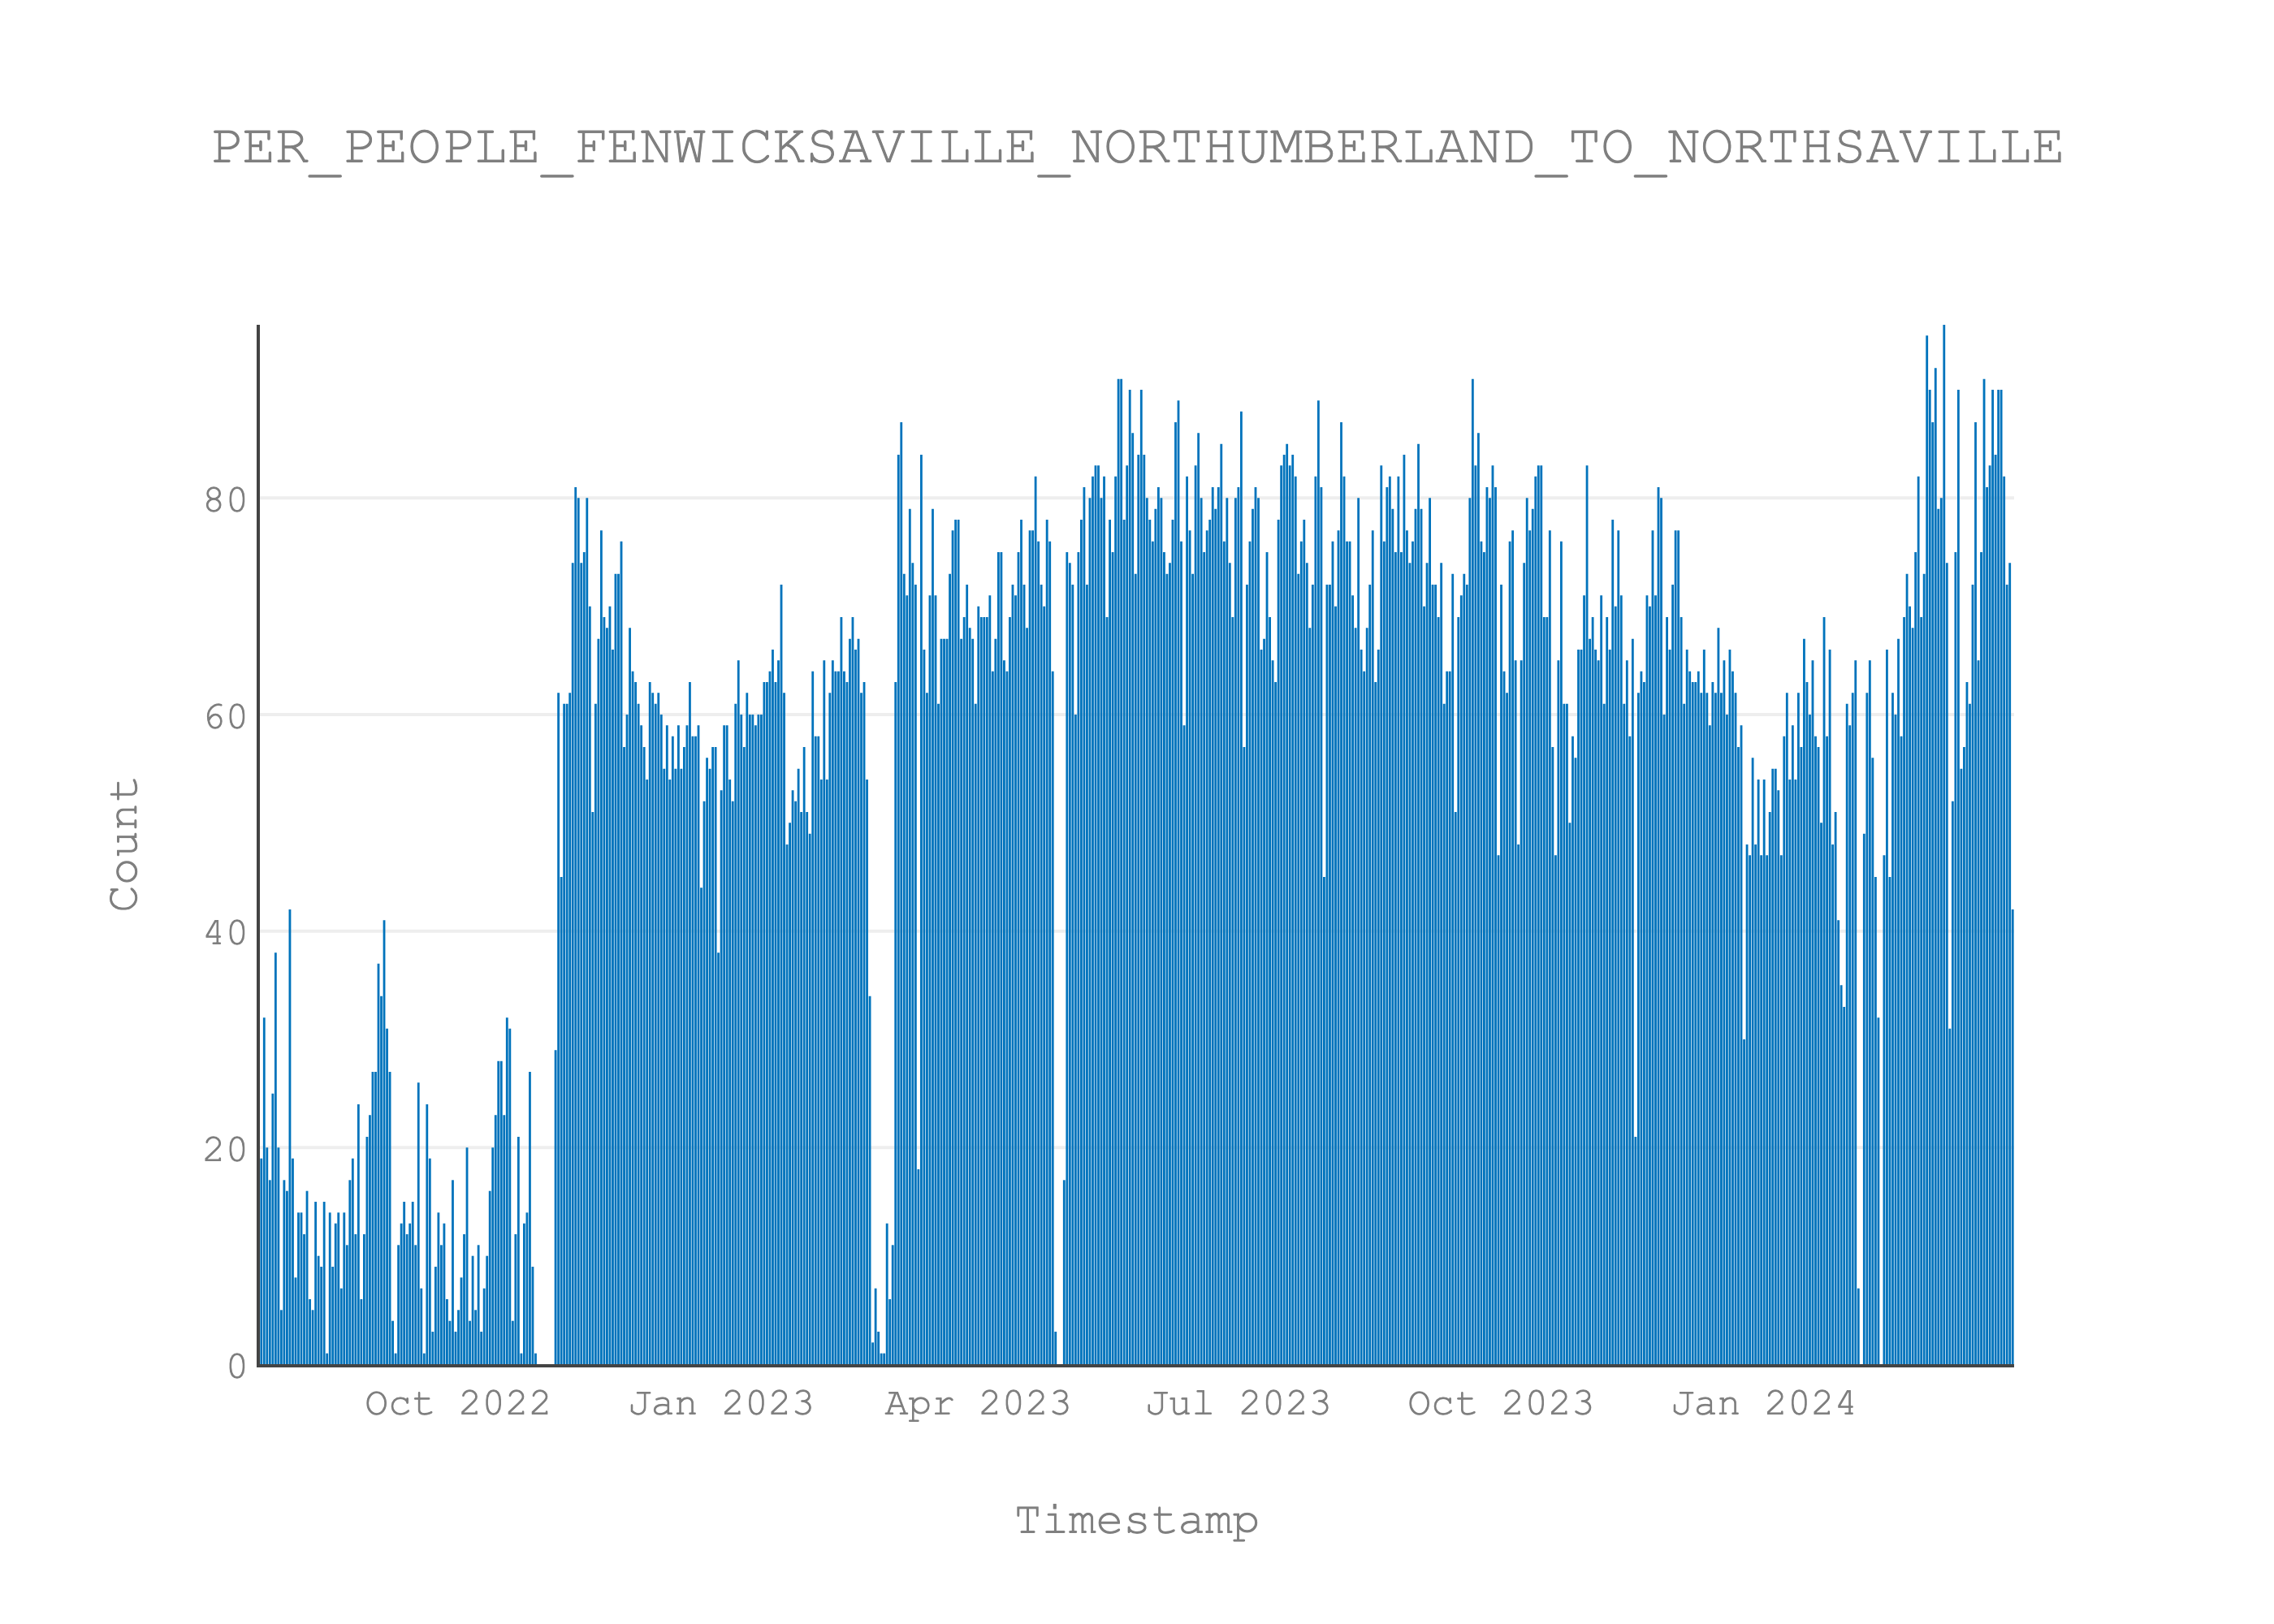
\includegraphics{figures/methodology/records_per_day_example.png}%
    }
    \caption{Example of records recorded per day}
    \label{fig:records_per_day_example}
\end{figure}

\subsubsection{Data Preprocessing}

Data preprocessing is essential to ensure optimal model performance. The neural networks need to be 'aware' of the data gaps to ensure that they are not training on the unrepresentative sequences. ML for time-series models assume that sequential data points are evenly sampled over time, however, imputing the missing data can affect it integrity. For this reason, the data has been left in its raw form, and a consecutive sequence detection and labelling algorithm has been developed (see Section \ref{subsubsection: imp_data_preprocessing}).

Figure \ref{fig:preprocessed_data_sequenced_example_timeseries} shows the outputs of the data preprocessing stage for the same sensor as above. Each new consecutive sequence is shown as a new colour. The sequences in this example a appear to restart with a daily pattern. This means each sequence is less than 96 records long which limits the length of training windows that can be used in the machine learning pipeline (this is explained further in Section \ref{subsubsection: des_data_loading}).


\begin{figure}[H]
    \centering
    \adjustbox{width=\linewidth, keepaspectratio}{%
        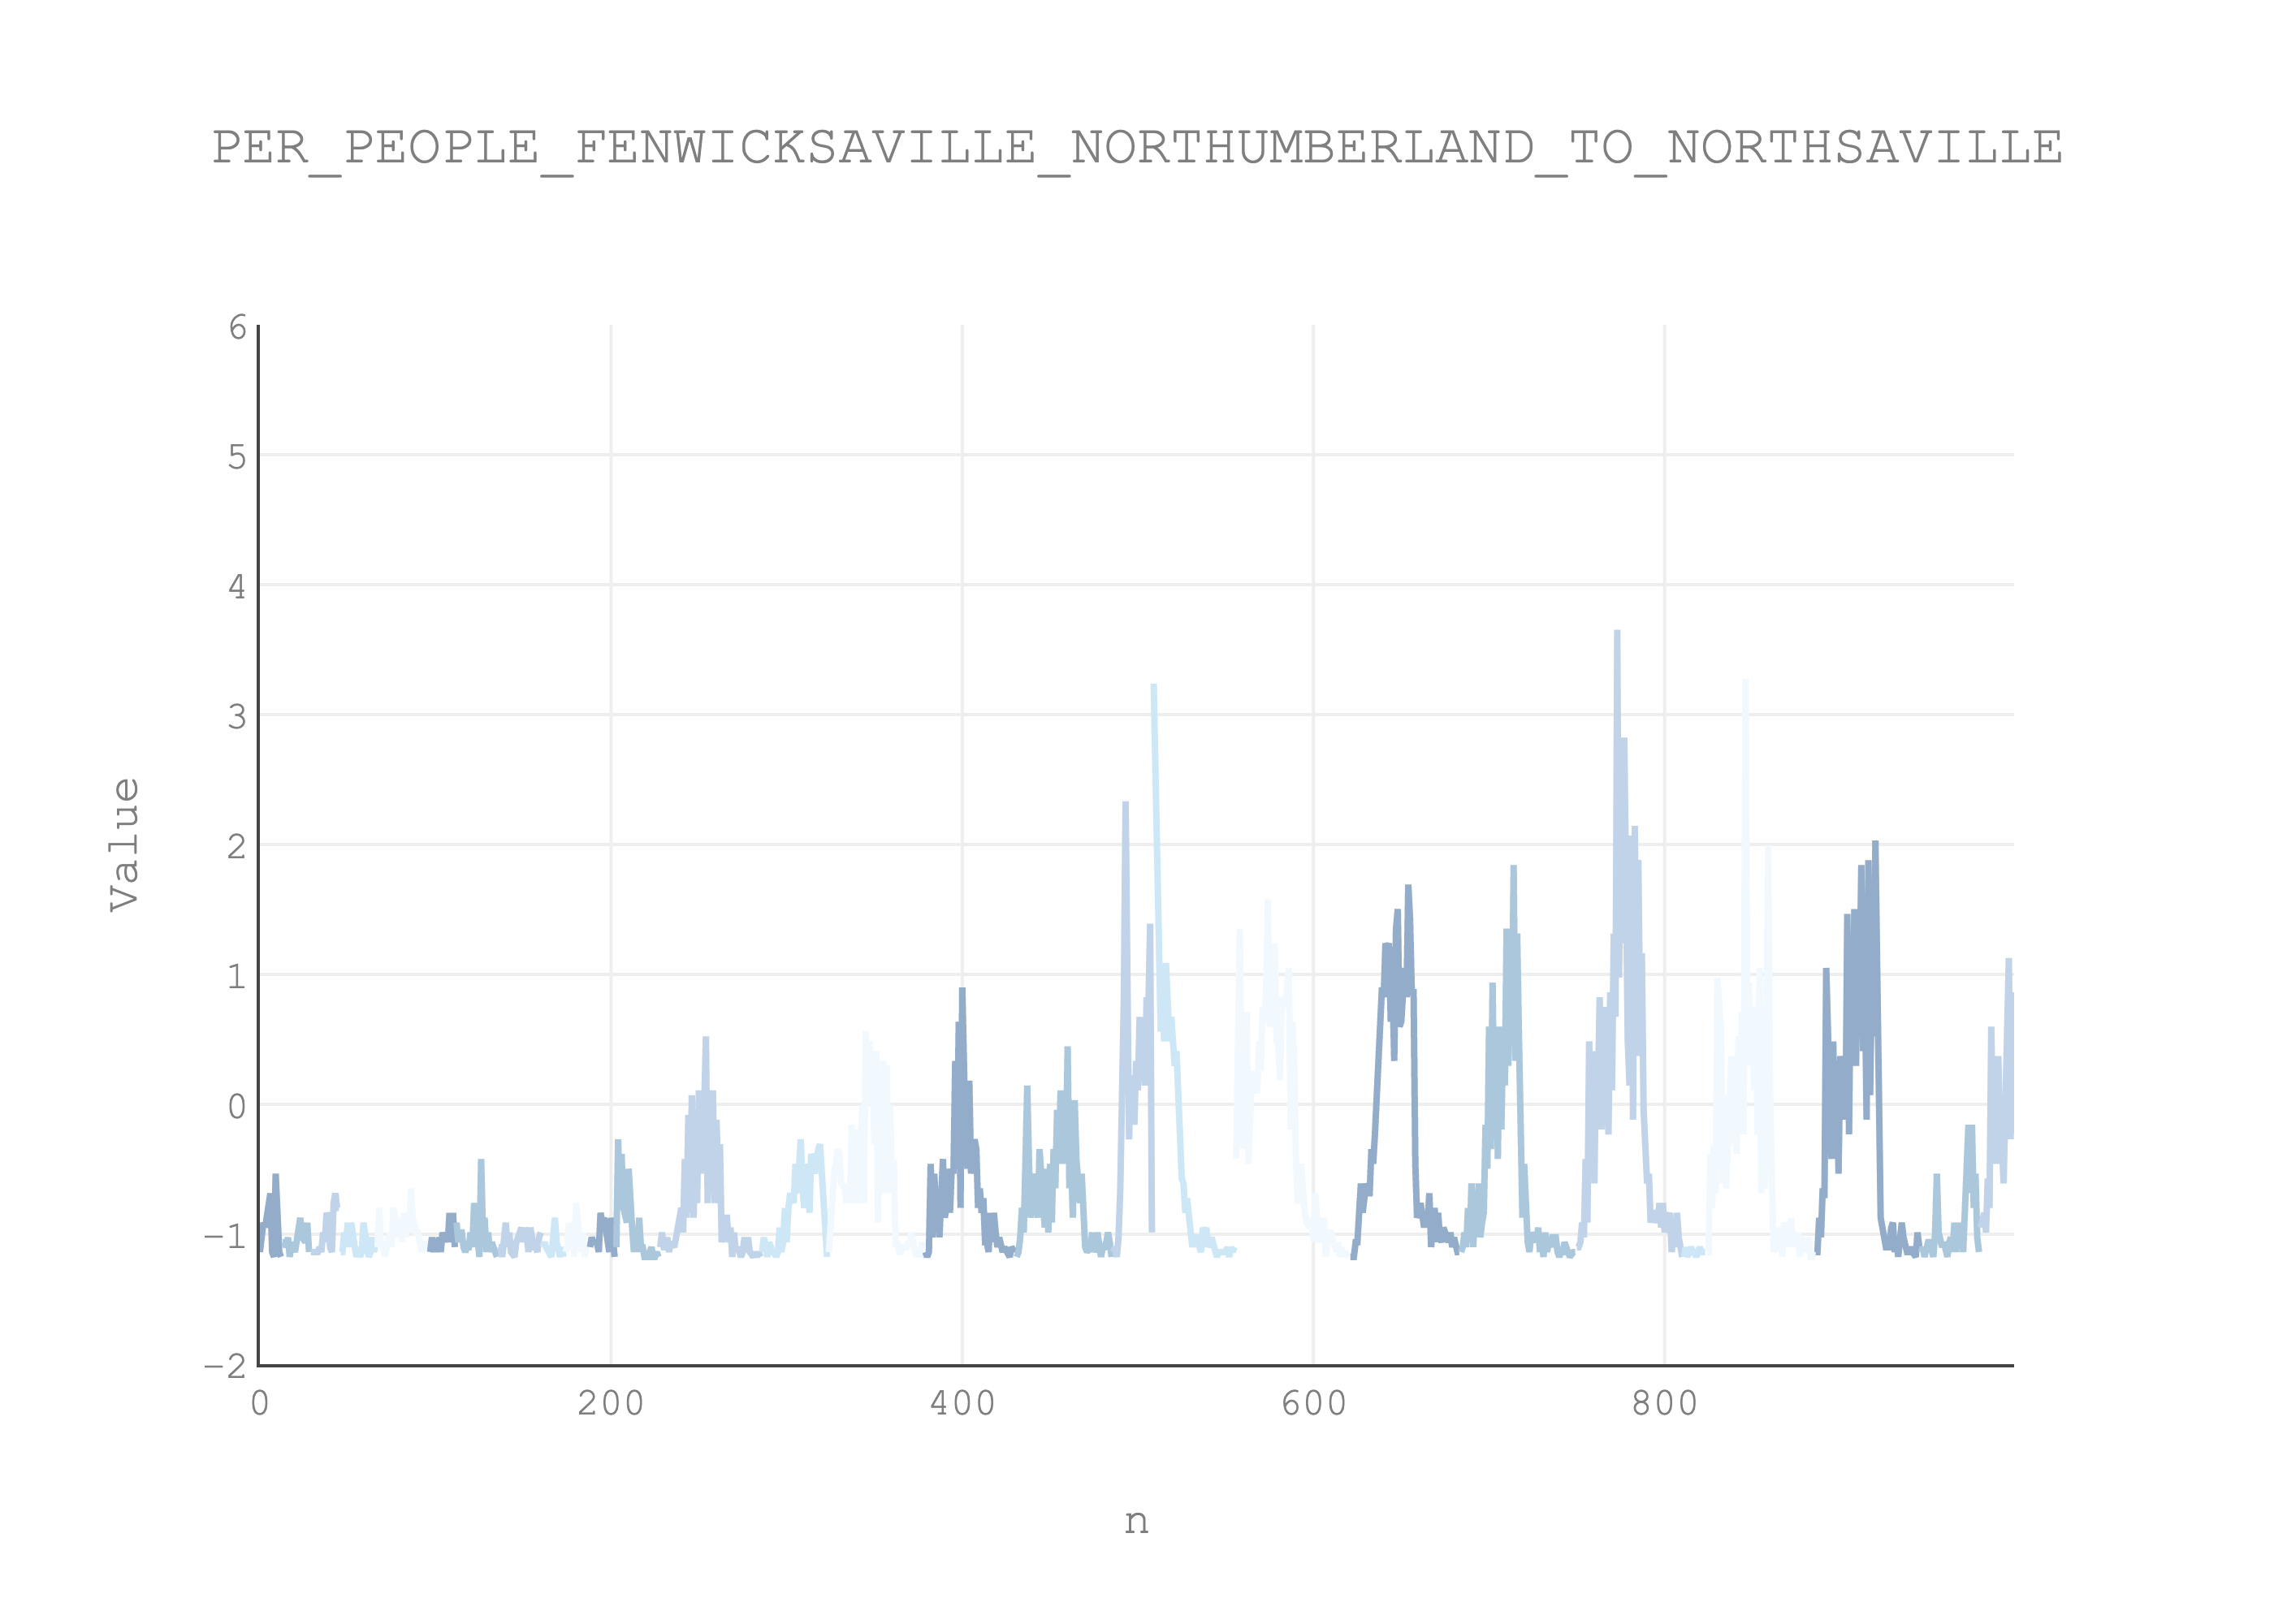
\includegraphics{figures/methodology/engineered_data_example_timeseries.png}%
    }
    \caption{Example of preprocessed data from a sensor}
    \label{fig:preprocessed_data_sequenced_example_timeseries}
\end{figure}

\subsubsection{Feature Engineering}

Feature engineering is the process of transforming raw data into features that can be used by machine learning algorithms. The features are engineered to capture the underlying patterns in the data. Figure \ref{fig:frequency_features_example_timeseries} shows an example of engineered frequency features from the same sensor shown previously (frequency features are shown as grey lines and the pedestrian flow data as blue). The uneven looking sinusoids highlight the missing data gaps. The features are calculated using a Lomb-Scargle Periodogram (similar to Fourier Transform but applicable to data with missing records).

The features are then normalised using the Standard Scaler equation shown in Equation \ref{eq:standardscaler}. The standard scalar normalisation technique is chosen to ensure that any future data points falling outside of the existing range can be scaled appropriately (a min max scaler would not be appropriate in this case). Calculating the mean and standard deviation in the scaling process also serves as a check for future data drift (because movement patterns change over the time the mean is likely to be non-stationary).

\begin{eqfloat}[H]
    \begin{equation}
        X'_i= \frac{X_i-\mu}{\sigma}
        \label{eq:standardscaler}
    \end{equation}
    \caption{Standard Scaler equation}
\end{eqfloat}

\begin{figure}[H]
    \centering
    \adjustbox{width=\linewidth, keepaspectratio}{%
        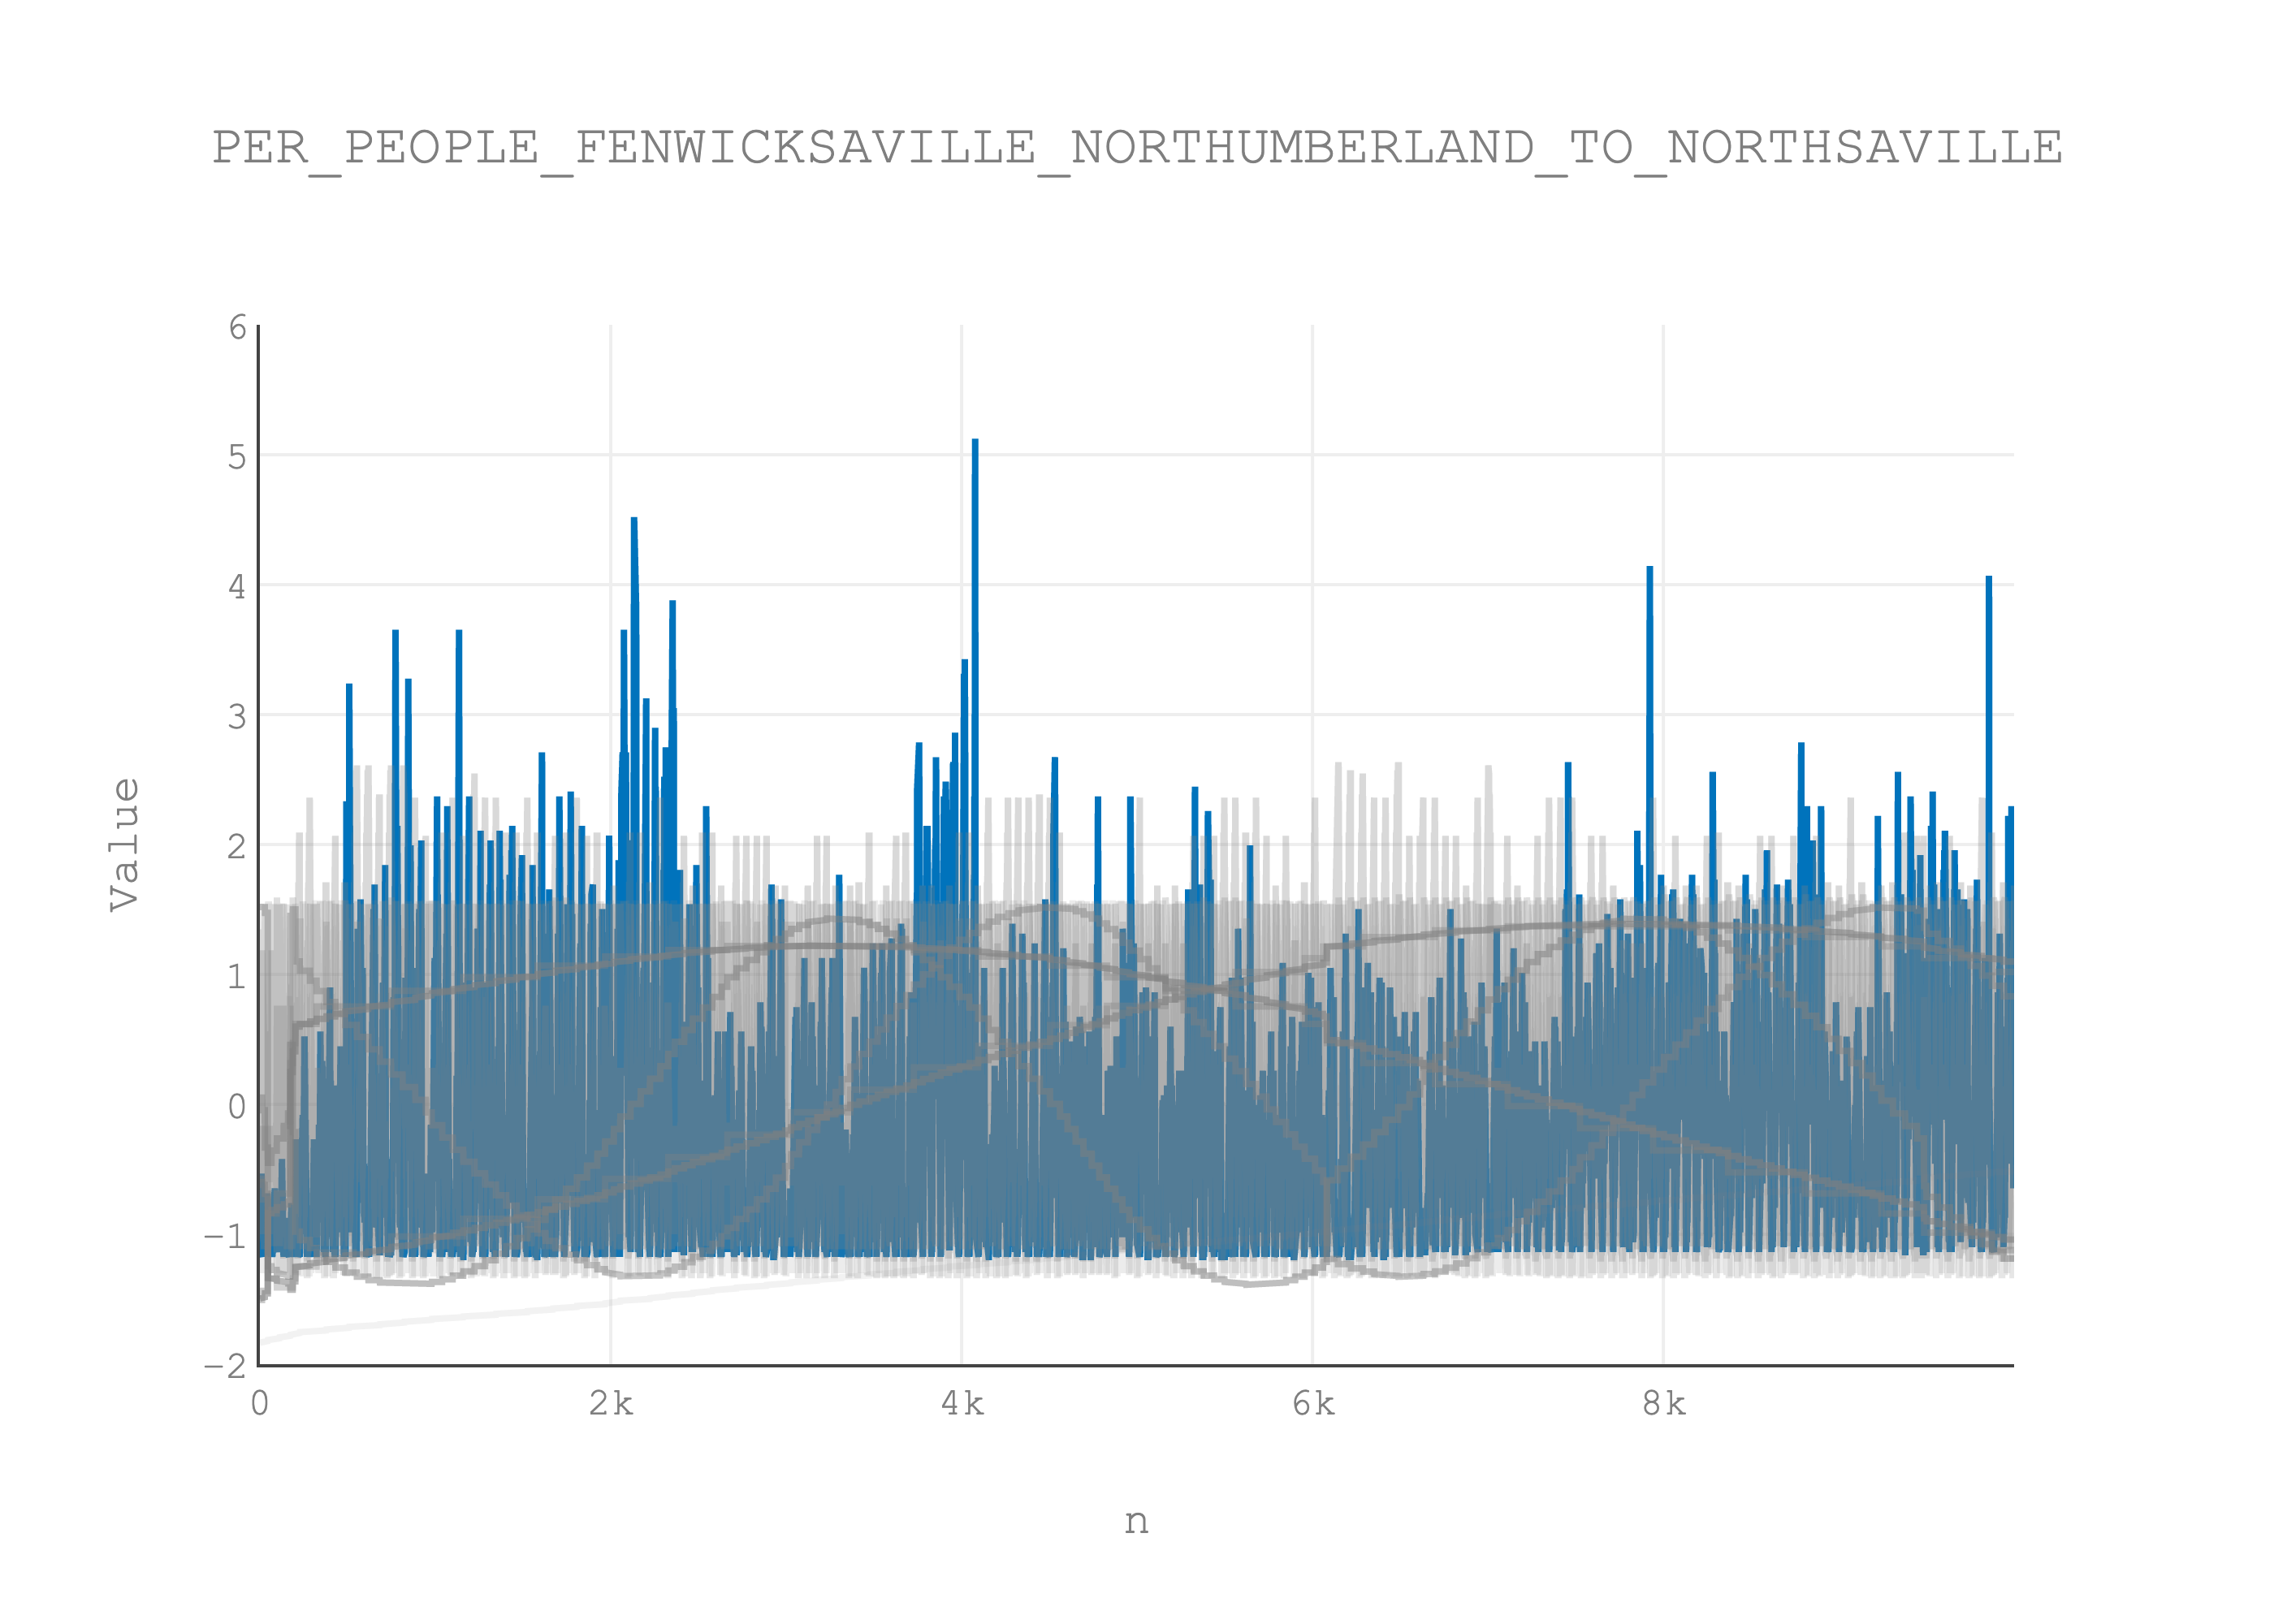
\includegraphics{figures/methodology/frequency_features_example_timeseries.png}%
    }
    \caption{Example of engineered frequency features from a sensor}
    \label{fig:frequency_features_example_timeseries}
\end{figure}


\subsection{Data Loading}
\label{subsubsection: des_data_loading}

For recurrent neural networks (such as LSTMs), the data must be windowed to create standard length sequences of data that can be used for training. An example window is shown in Figure \ref{fig:dataloader_example_training_sequence}. Each window is contains a sequence of data points from a sensor (shown in blue) and a number of additional sequences from engineering features (show in grey). The length of this window is set as a hyper-parameter. The label (shown in red) for each window is the data point a specified number of time steps into the future (the horizon). The window size variable is a hyper-parameter that can be tuned to improve the performance of the model. The horizon hyper-parameter also affects the models performance, but more importantly, the horizon dictates how far into the future the model can predict. In the example plot, the window size is 4 and the horizon is 8. This means that the model is recursively trained to predict the pedestrian flow 8 time steps (2 hours) into the future using the previous 4 time steps (1 hour) of data.

\begin{figure}[H]
    \centering
    \adjustbox{width=\linewidth, keepaspectratio}{%
        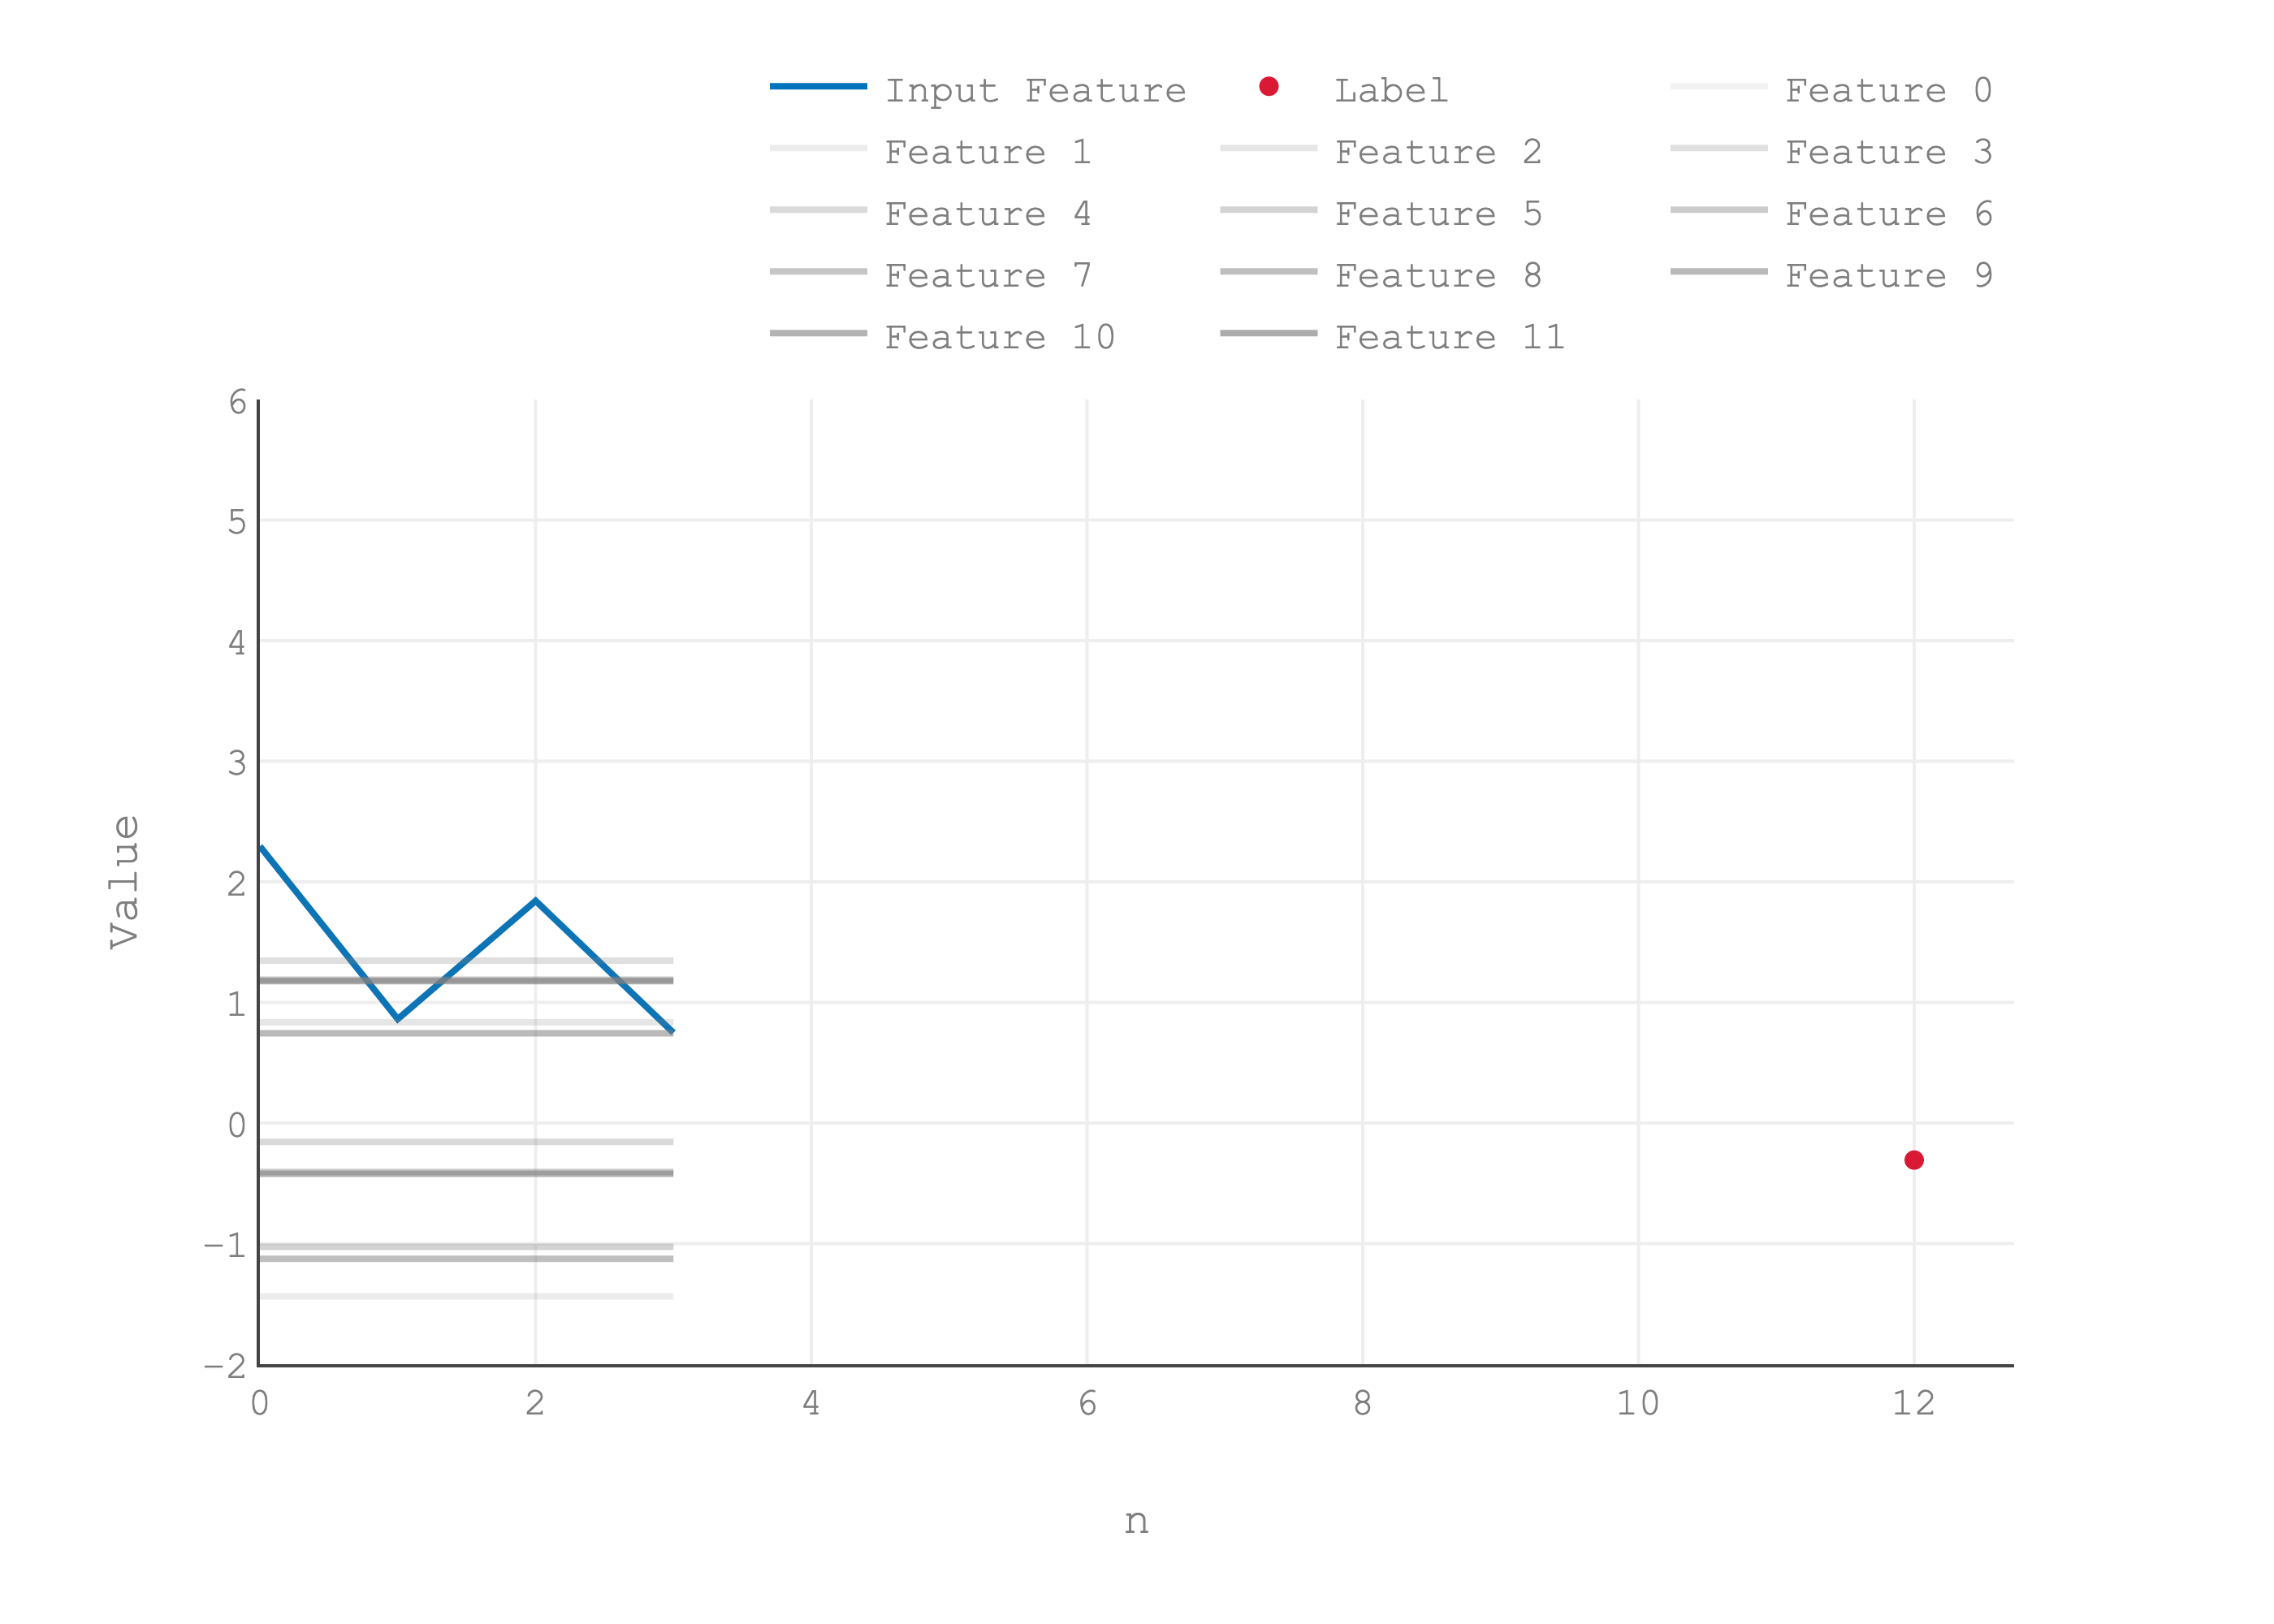
\includegraphics{figures/methodology/dataloader_example_training_sequence.png}%
    }
    \caption{Examples of data quality issues in the urban observatory}
    \label{fig:dataloader_example_training_sequence}
\end{figure}

\subsubsection{Model Training}

LSTMs (long-short term memory units) and GRUs (gated recurrent units) are well regarded in scientific literature for their ability to capture long-term dependencies in sequential data and have therefore been chosen for this research. The LSTM (Figure \ref{fig:lstm}) is a more complex model than the GRU (Figure \ref{fig:gru}) and has more parameters. Both models are types of recurrent neural networks (Figure \ref{fig:rnn}) that have been designed to overcome the vanishing/exploding gradients problem. The basic idea behind RNNs is that the neural network is updated with each new recurrent sequence. A standard RNN consists of layers of neurons that are connected to each other. The output of each neuron is fed back into the network at the next time step. This allows the network to learn the temporal dependencies in the data. The problem with standard RNNs is that they have difficulty learning long-term dependencies. The LSTM and GRU models have been designed to overcome this issue through the addition of gates and memory cells (additional neurons that store information about the sequence). The LSTM has three gates (input, output, and forget) and the GRU has two gates (reset and update).

\begin{figure}[H]
    \centering
    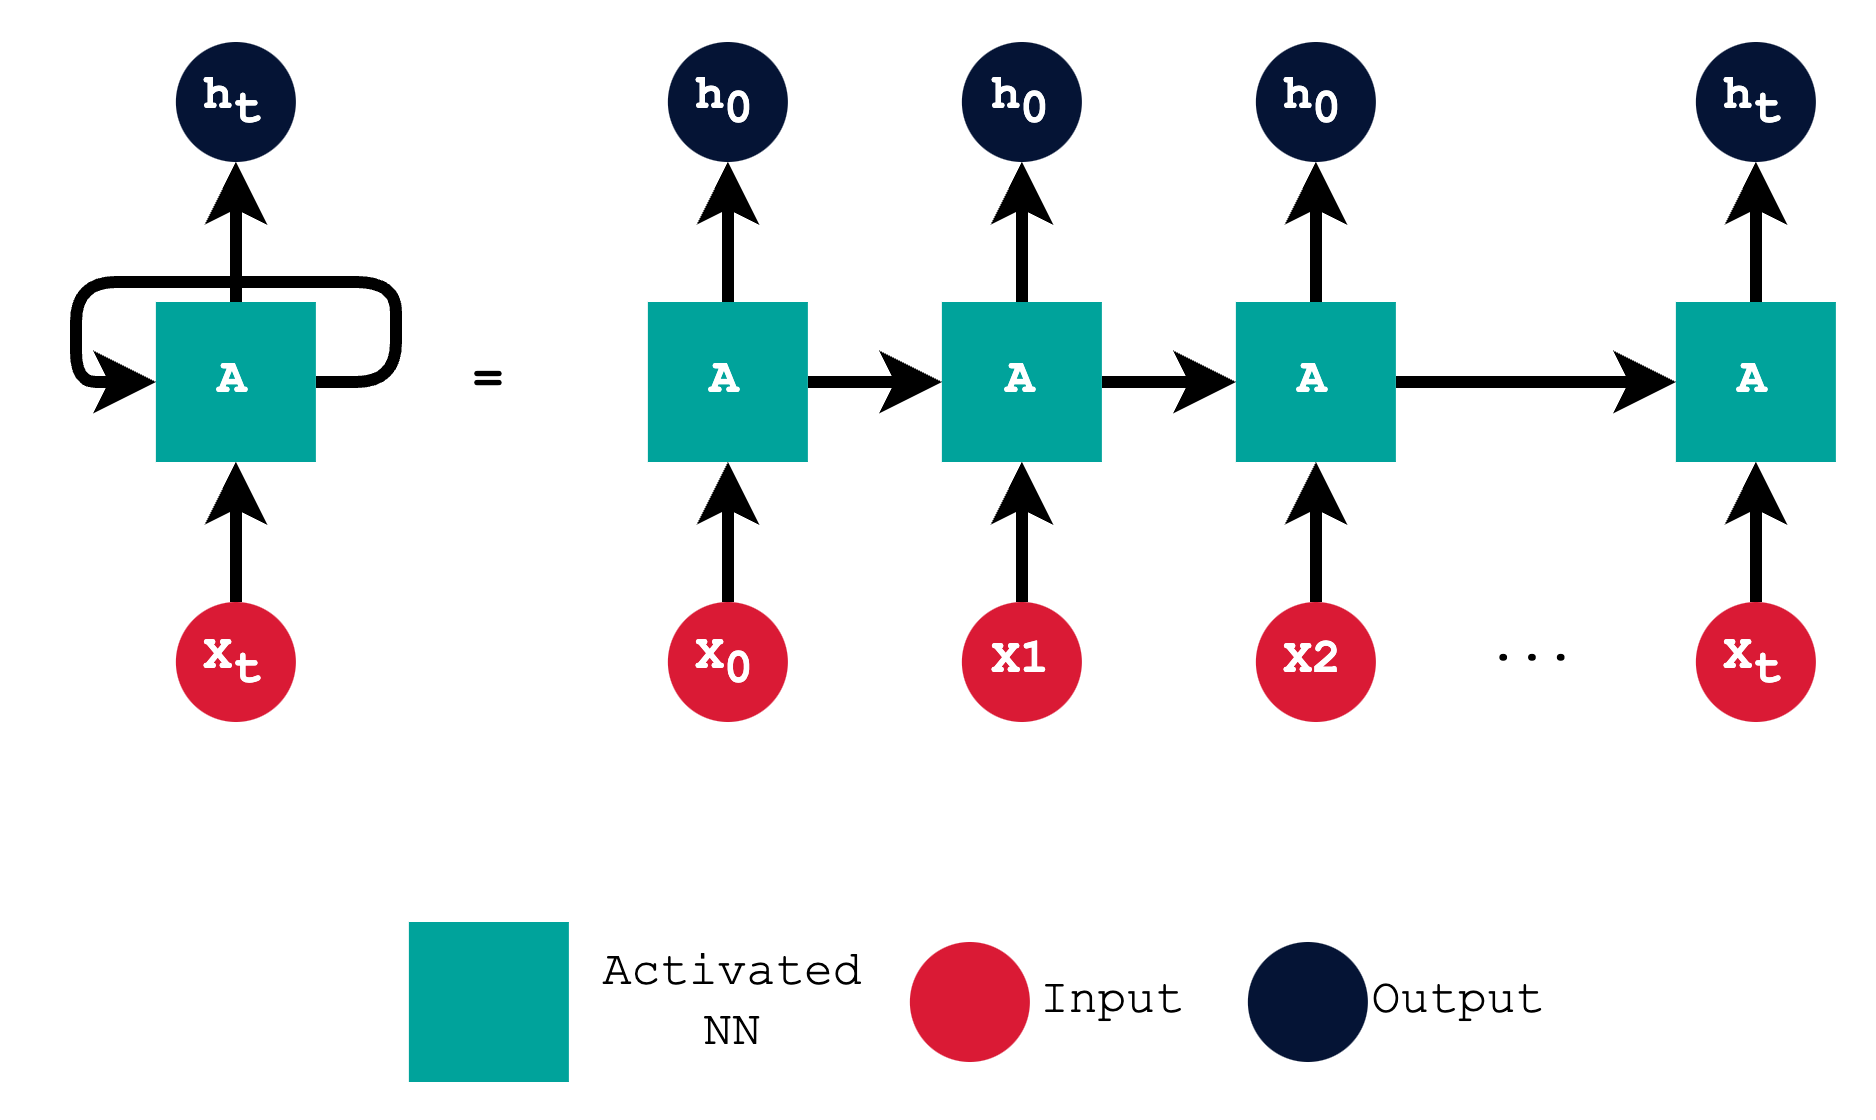
\includegraphics[scale=0.15]{figures/methodology/rnn.png}
    \caption{Recurrent neural network (RNN) architecture}
    \label{fig:rnn}
\end{figure}

\begin{figure}[H]
    \centering
    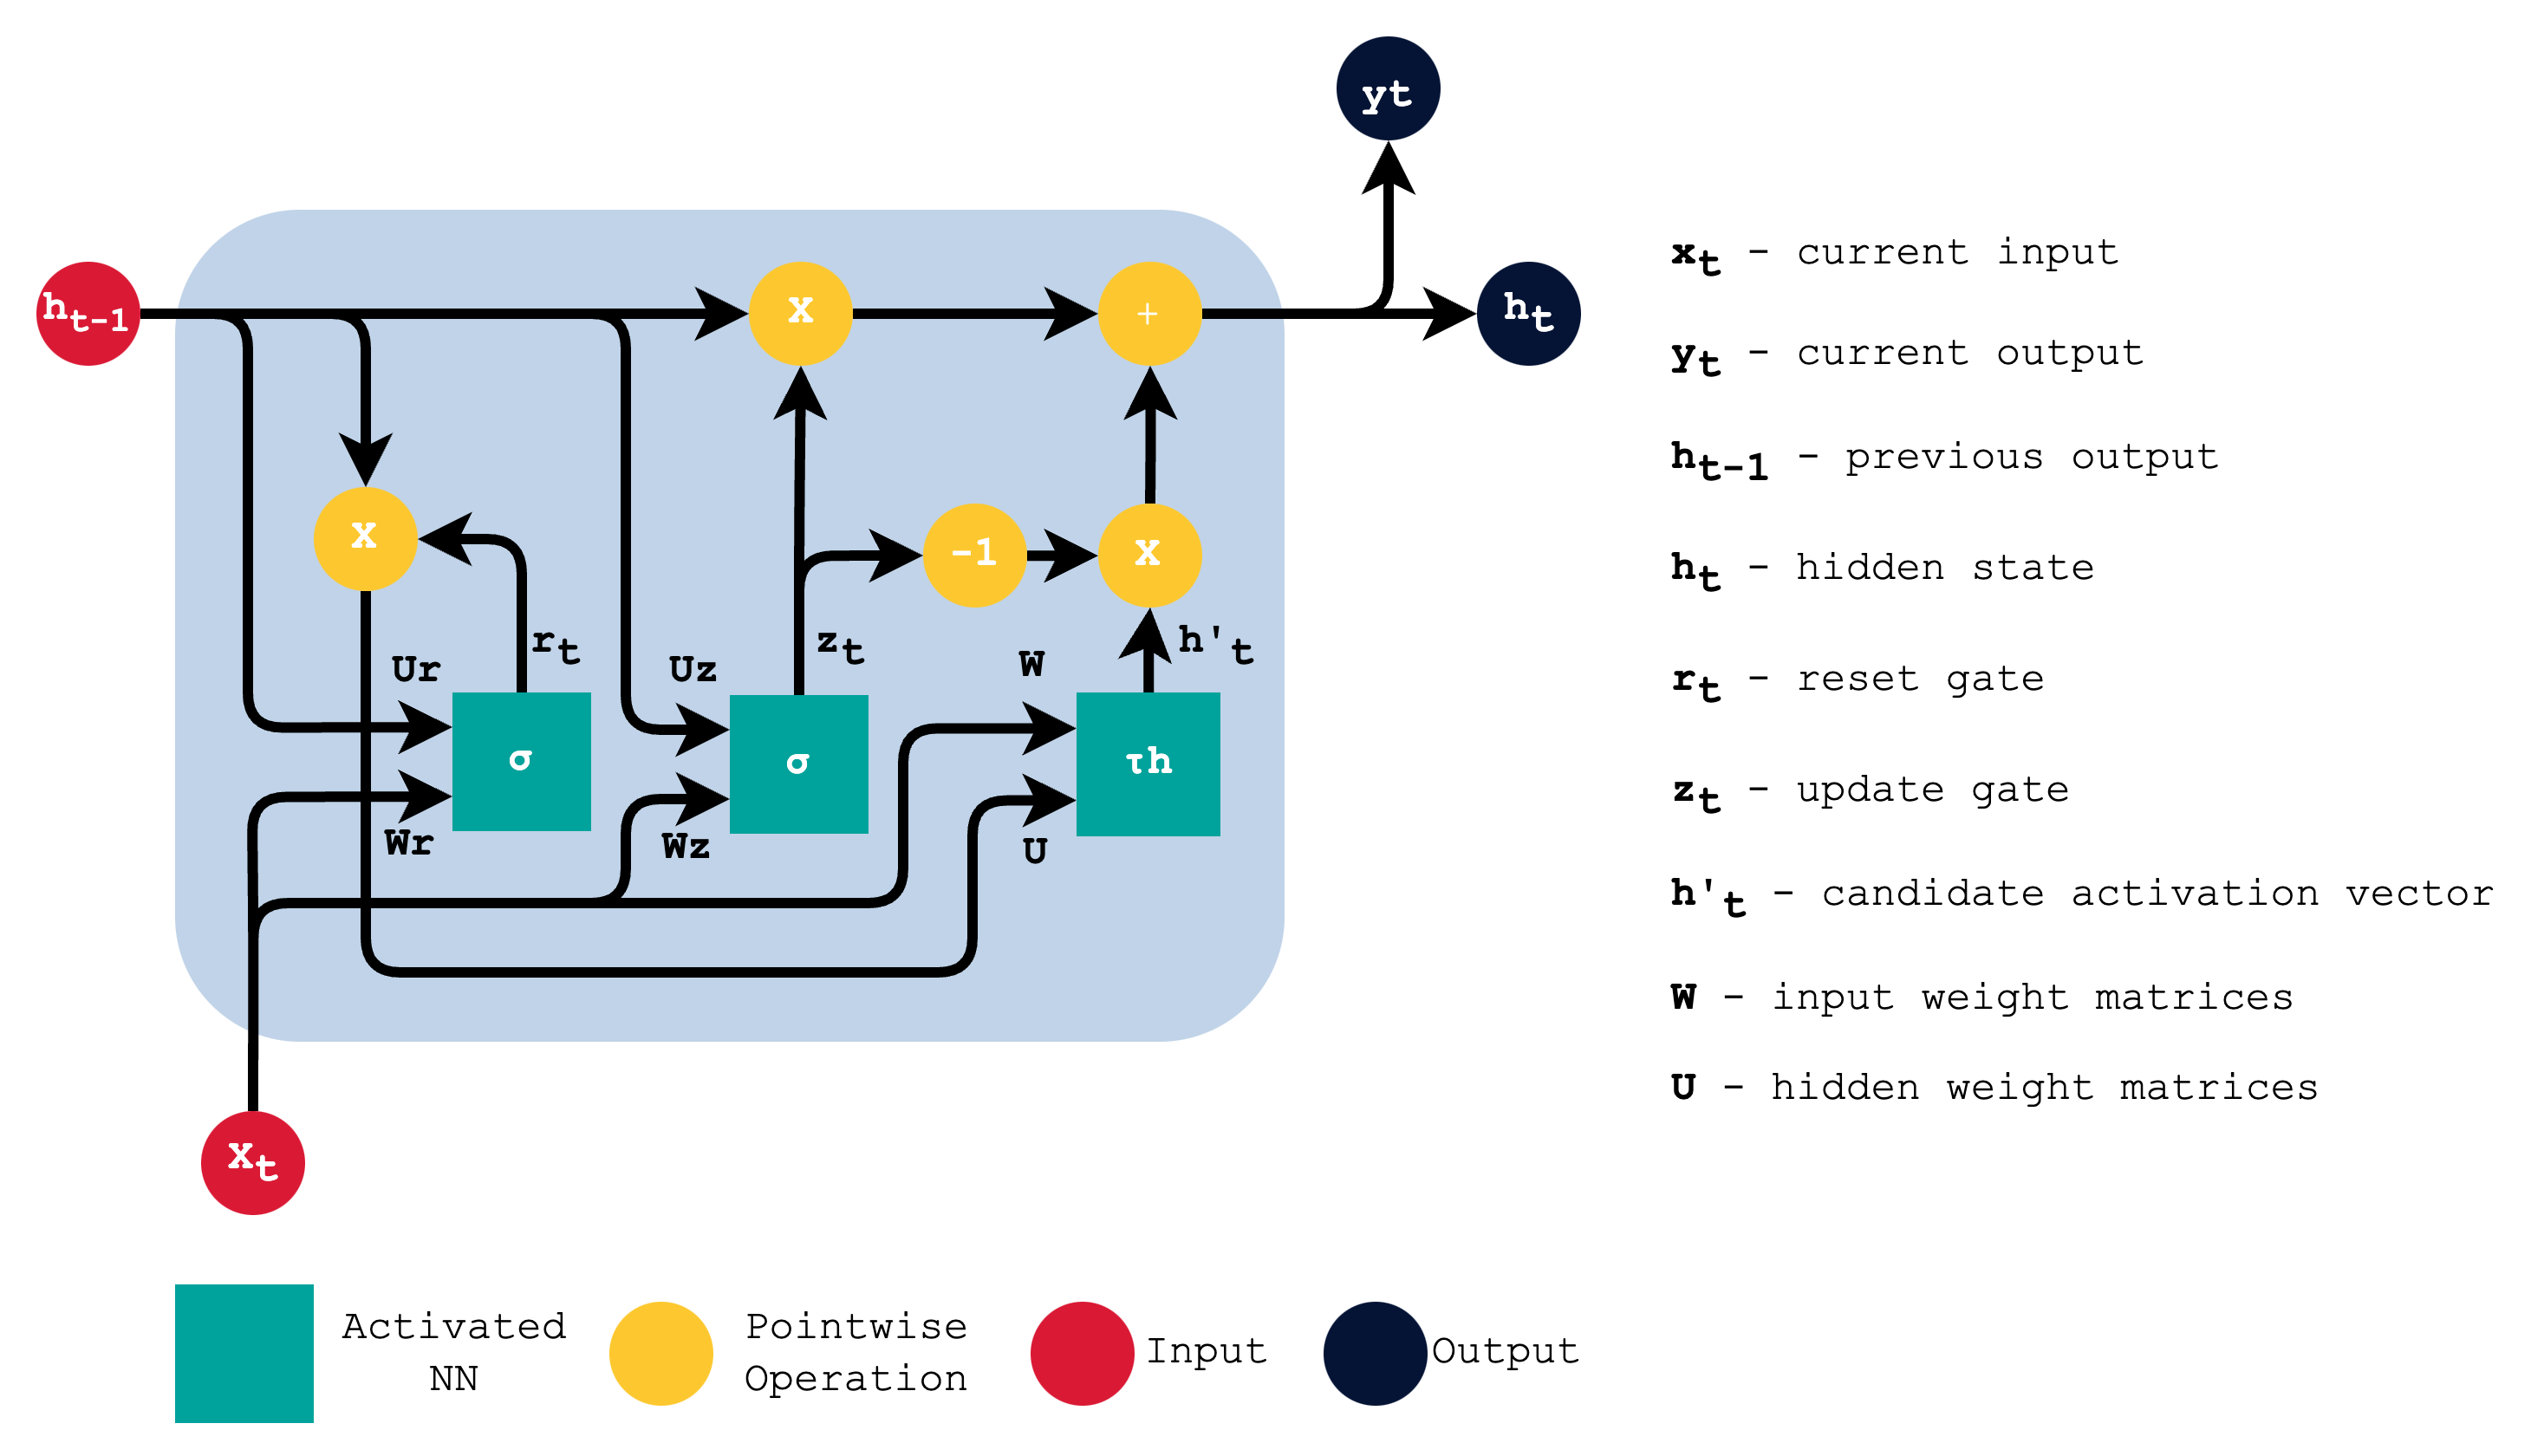
\includegraphics[scale=0.15]{figures/methodology/gru.png}
    \caption{Gated recurrent unit (GRU) architecture}
    \label{fig:gru}
\end{figure}

\begin{figure}[H]
    \centering
    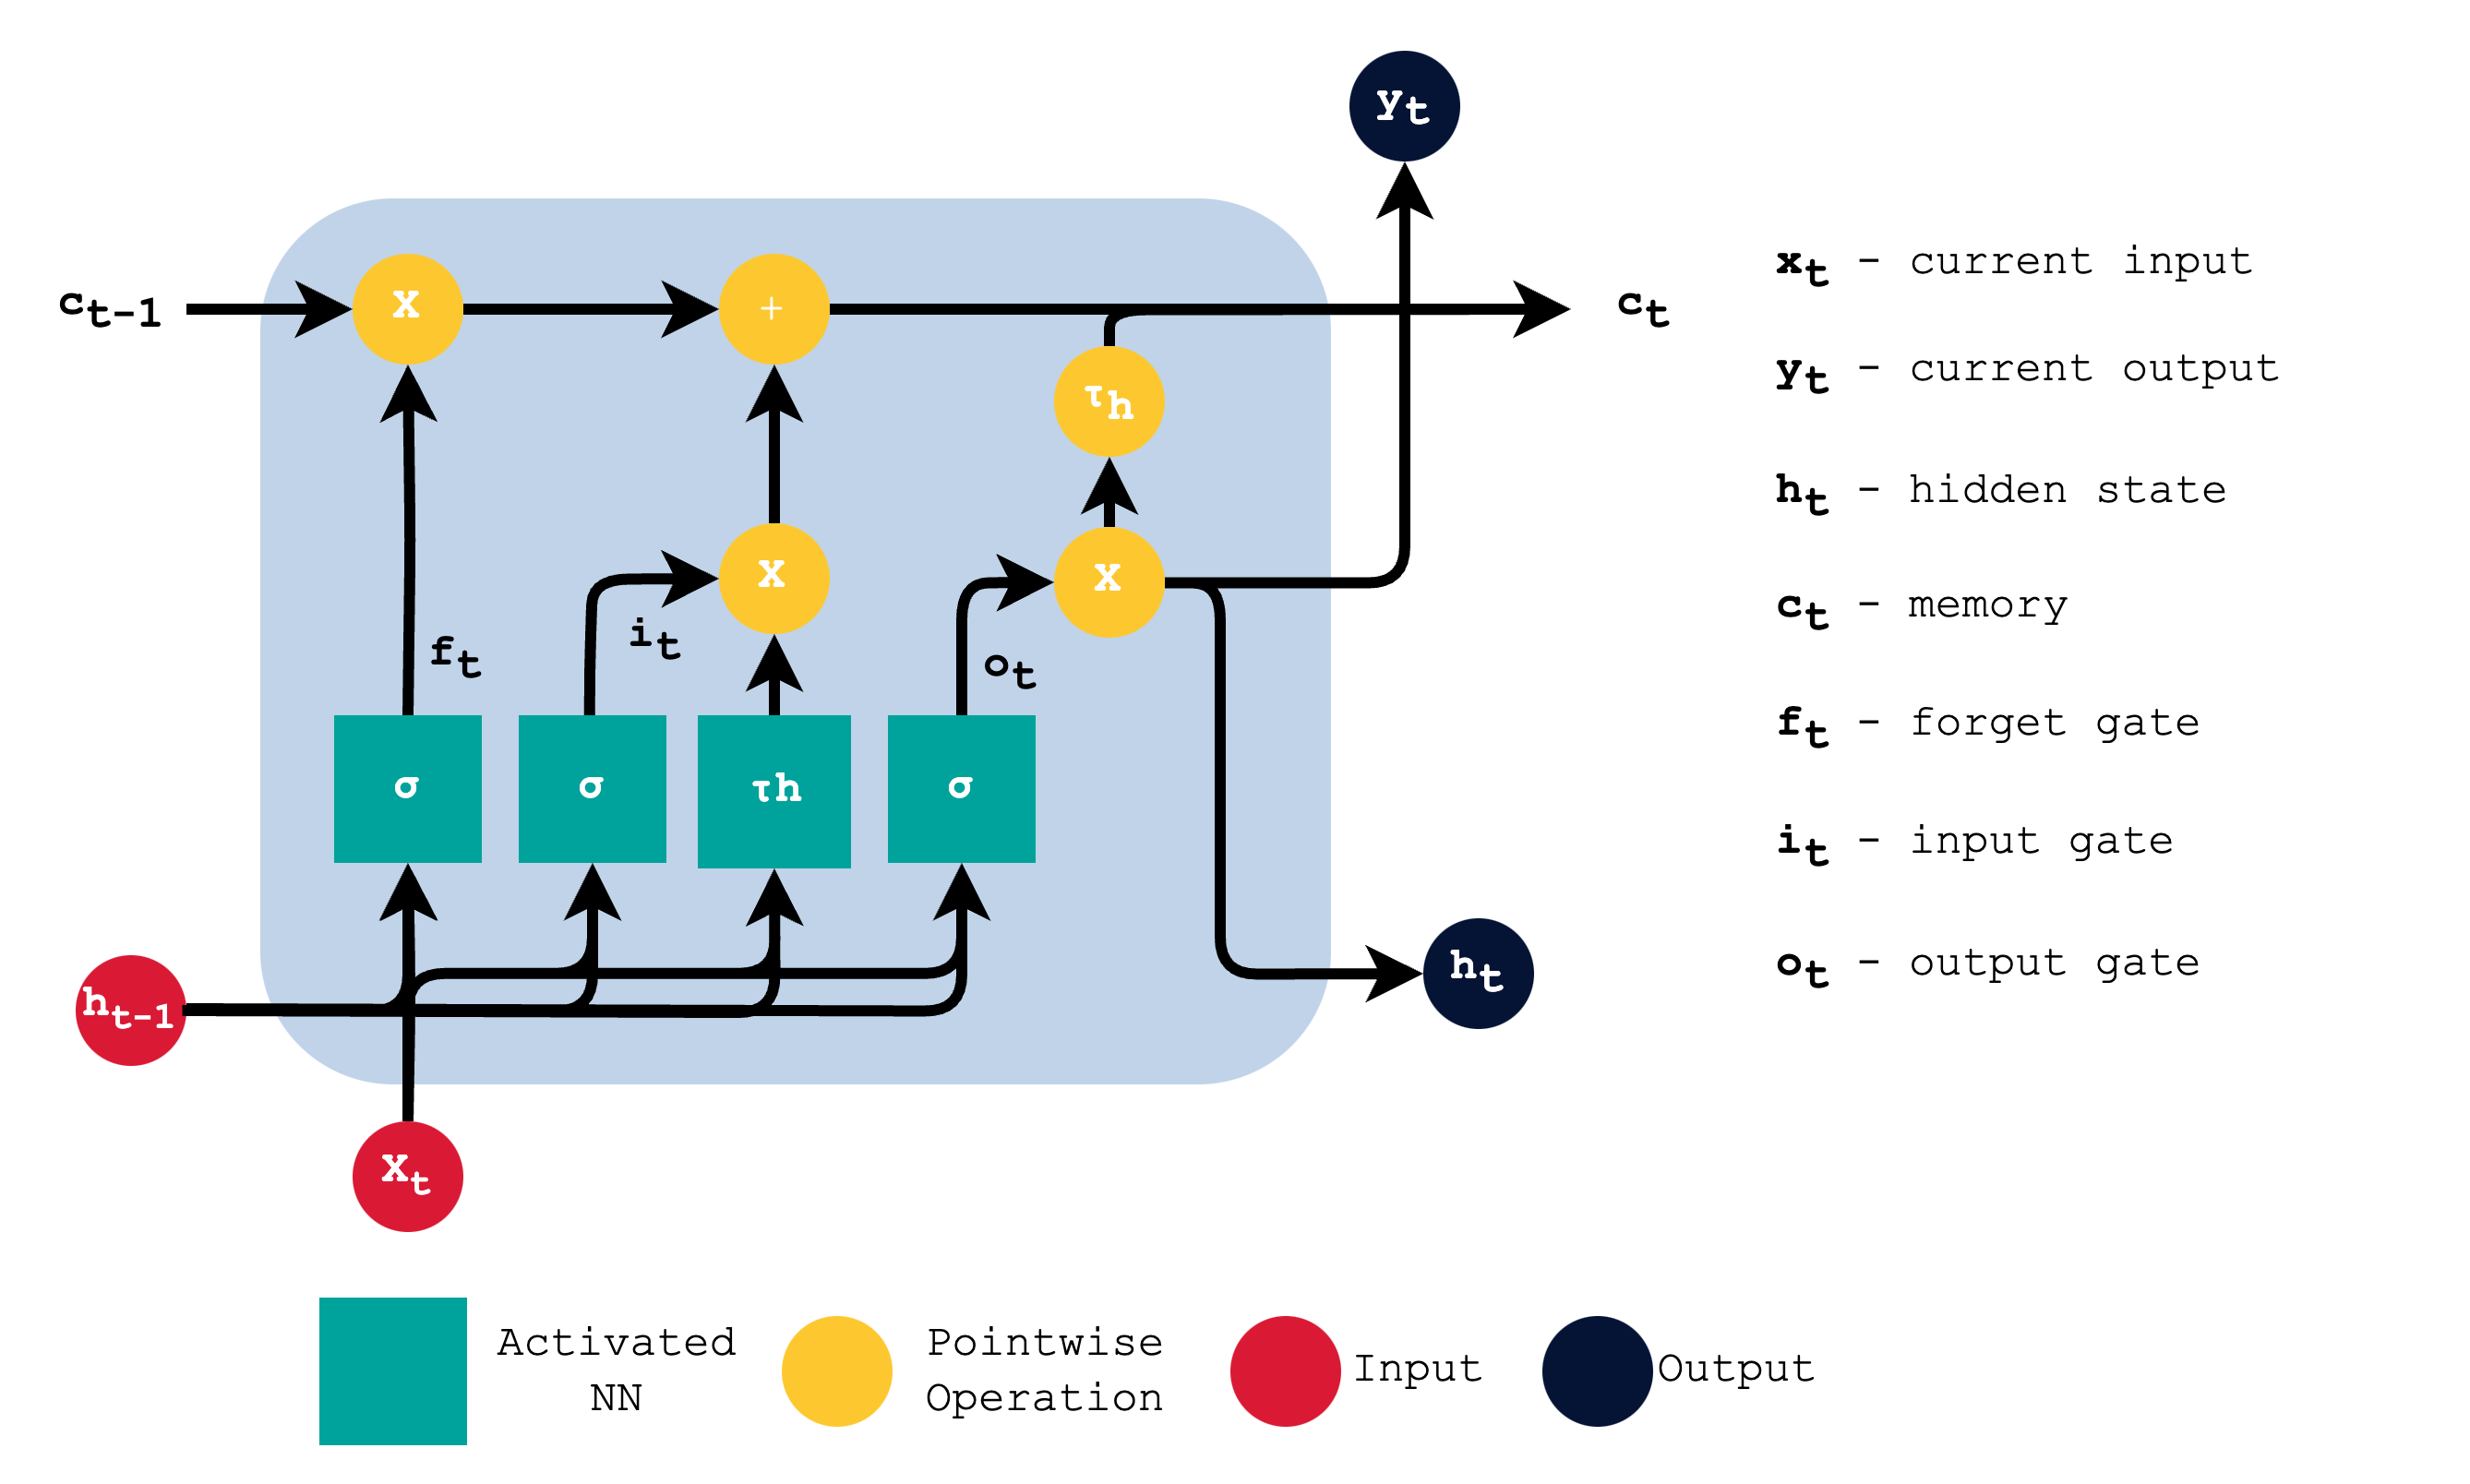
\includegraphics[scale=0.15]{figures/methodology/lstm.png}
    \caption{Long short-term memory (LSTM) architecture}
    \label{fig:lstm}
\end{figure}

A number of hyper-parameters have been used in training the models. An overview and explanation is provided here, with a full list of the implemented hyper-parameters and their values provided in table \ref{tab:hyperparameters}. Some values that could be considered hyper-parameters but will not be tuned in this research are listed in the preset hyper-parameters section below. The hyper-parameters that will be tuned are split into two categories: data hyper-parameters and model hyper-parameters. The data hyper-parameters are those that affect the structure of the data used in the model training process. The model hyper-parameters are those that affect the architecture of the model itself.

\textbf{Preset hyper-parameters (data):}
\begin{itemize}
    \item \textbf{Length of time-series} - the number of time steps available for training the model. This varies depending on the sensor and the data quality issues present in the data. Whilst this could be restricted to a fixed number of data points, the aim of the experiment is to train the model on as much data as possible in order to understand the effect of data quality on the model performance. Therefore a fixed time period is used instead.
    \item \textbf{Optimiser} - whilst experimenting with different optimisers (e.g. Adam, RMSprop, SGD with momentum) can lead to different convergence behaviours, Adam will be used as the preset optimiser for this project to avoid high dimensionality during hyperparameter tuning.
    \item \textbf{Activation function} - LSTMs and GRUs have their own internal activation functions typically using a combination of sigmoid and tanh. As the required outputs of the models are continuous, no activation function is used on the output layer.
    \item \textbf{Loss function} - Mean squared error (MSE) will be used as the preset loss function for this project. This is a common loss function for regression problems is being used to avoid high dimensionality during hyperparameter tuning.
\end{itemize}

\textbf{Tuneable hyper-parameters (data):}
\begin{itemize}
    \item \textbf{Window size} - the number of time steps used in each training window. A large window size can cause the model to overfit the data. A small window size can cause the model to under-fit the data.
    \item \textbf{Batch size} - the number of samples used in each iteration of training. A large batch size can cause the model to converge too quickly and miss the global minimum. A small batch size can cause the model to take too long to converge.
    \item \textbf{Horizon} - the number of time steps into the future the model is trained to predict. A large horizon is more difficult to predict and can lead to overfitting. A small horizon is much easier and often leads to under-fitting (the model learns to predict the last data point in the sequence).
\end{itemize}

\textbf{Tuneable hyper-parameters (model):}
\begin{itemize}
    \item \textbf{Number of hidden units} - this determines the capacity and complexity of the model. More units can capture more complex patterns in the data, but may lead to overfitting.
    \item \textbf{Number of layers} - deeper networks can learn more abstract representations but are harder to train and more prone to overfitting.
    \item \textbf{Epochs} - complete passes through the training data. Too few epochs generally lead to under-fitting, and too many can result in overfitting.
    \item \textbf{Learning rate} - this controls how quickly the model parameters are updated. during training. It's crucial for convergence and avoiding local optima. A high learning rate can cause the model to miss the global minimum. A low learning rate can cause the model to take too long to converge.
    \item \textbf{Dropout rate} - this is a regularisation technique that can help to prevent overfitting, the dropout rate determines how many units are randomly 'dropped' during training.
\end{itemize}

\subsubsection{Model Evaluation}

To evaluate the model a range of metrics will be used. The primary metric will be the root mean squared error (RMSE) shown in equation \ref{eq:rmse}. RMSE measures the difference between the predicted and actual values and is more sensitive to outliers than the mean absolute error (MAE). Mean absolute percentage error (MAPE) shown in equation \ref{eq:mape} and R-squared (R$^2$) metric shown in equation \ref{eq:rsquared} will also be used. R$^2$ measures the proportion of the variance in the dependent variable that is predictable from the independent variable(s).

\begin{itemize}
    \item Model evaluation - what metrics are used?
\end{itemize}

\begin{eqfloat}[H]
    \begin{equation}
        \text{RMSE} = \sqrt{\frac{1}{n}\sum_{i=1}^{n}(y_i - \hat{y}_i)^2}
        \label{eq:rmse}
    \end{equation}
    \caption{Root mean squared error (RMSE)}
\end{eqfloat}

\begin{eqfloat}[H]
    \begin{equation}
        \text{MAPE} = \frac{1}{n}\sum_{i=1}^{n}\left|\frac{y_i - \hat{y}_i}{y_i}\right|
        \label{eq:mape}
    \end{equation}
    \caption{Mean absolute percentage error (MAPE)}
\end{eqfloat}

\begin{eqfloat}[H]
    \begin{equation}
        \text{R}^2 = 1 - \frac{\sum_{i=1}^{n}(y_i - \hat{y}_i)^2}{\sum_{i=1}^{n}(y_i - \bar{y})^2}
        \label{eq:rsquared}
    \end{equation}
    \caption{R-squared (R$^2$)}
\end{eqfloat}

\subsection{Research Implementation} \label{implementation}

The research will be implemented using Python and various libraries such as Pandas, NumPy, and PyTorch. This system has been developed in a modular fashion to allow for easy integration of new sensors, data sources, models, and data transformation steps. A full description of the implementation methodology is provided in the package documentation which can be found \href{https://carrowmw.github.io/phd-project/pipeline_module/overview/#}{here}.

An overview of each stage is provided below:

\subsubsection{Machine Learning Pipeline Development}

A list of hyper-parameters used in the machine learning pipeline is shown in Table \ref{tab:hyperparameters}. The ranges shown reflect the values that were used in the hyperparameter tuning process.

\begin{table}[h]
    \centering
    \scriptsize
    \begin{tabular}{|l|l|l|}
        \hline
        \textbf{Parameter} & \textbf{Suggestion Type} & \textbf{Value Range/Options} \\
        \hline
        window\_size       & suggest\_int             & 2 to 10                      \\
        \hline
        horizon            & suggest\_int             & 1 to 12                      \\
        \hline
        batch\_size        & suggest\_categorical     & [32, 64, 128]                \\
        \hline
        lr                 & suggest\_loguniform      & 1e-5 to 1e-1                 \\
        \hline
        epochs             & suggest\_int             & 5 to 50                      \\
        \hline
        model\_type        & suggest\_categorical     & ["lstm", "gru"]              \\
        \hline
        hidden\_dim        & suggest\_int             & 32 to 256                    \\
        \hline
        num\_layers        & suggest\_int             & 1 to 3                       \\
        \hline
        dropout            & suggest\_uniform         & 0.0 to 0.5                   \\
        \hline
    \end{tabular}
    \caption{Hyper-parameter tuning configuration}
    \label{tab:hyperparameters}
\end{table}

To tune the models hyper-parameters, the Optuna library was used in conjunction with MLflow for experiment tracking. The hyper-parameter tuning process is shown in Figure \ref{fig:hyperparameter_tuning}. The process involves involves running the pipeline multiple times with different hyper-parameters and recording the results. As the pipeline outputs as many models as there are sensors, the hyper-parameter tuning takes the average performance of all the models (an alternative approach would be to tune each sensor/model separately). R-squared was used as the metric for hyper-parameter tuning (this needs to switched to RMSE, MAPE, Loss weighted 1.0, 0.2, 0.1 and potentially normalised first).

\begin{figure}[H]
    \centering
    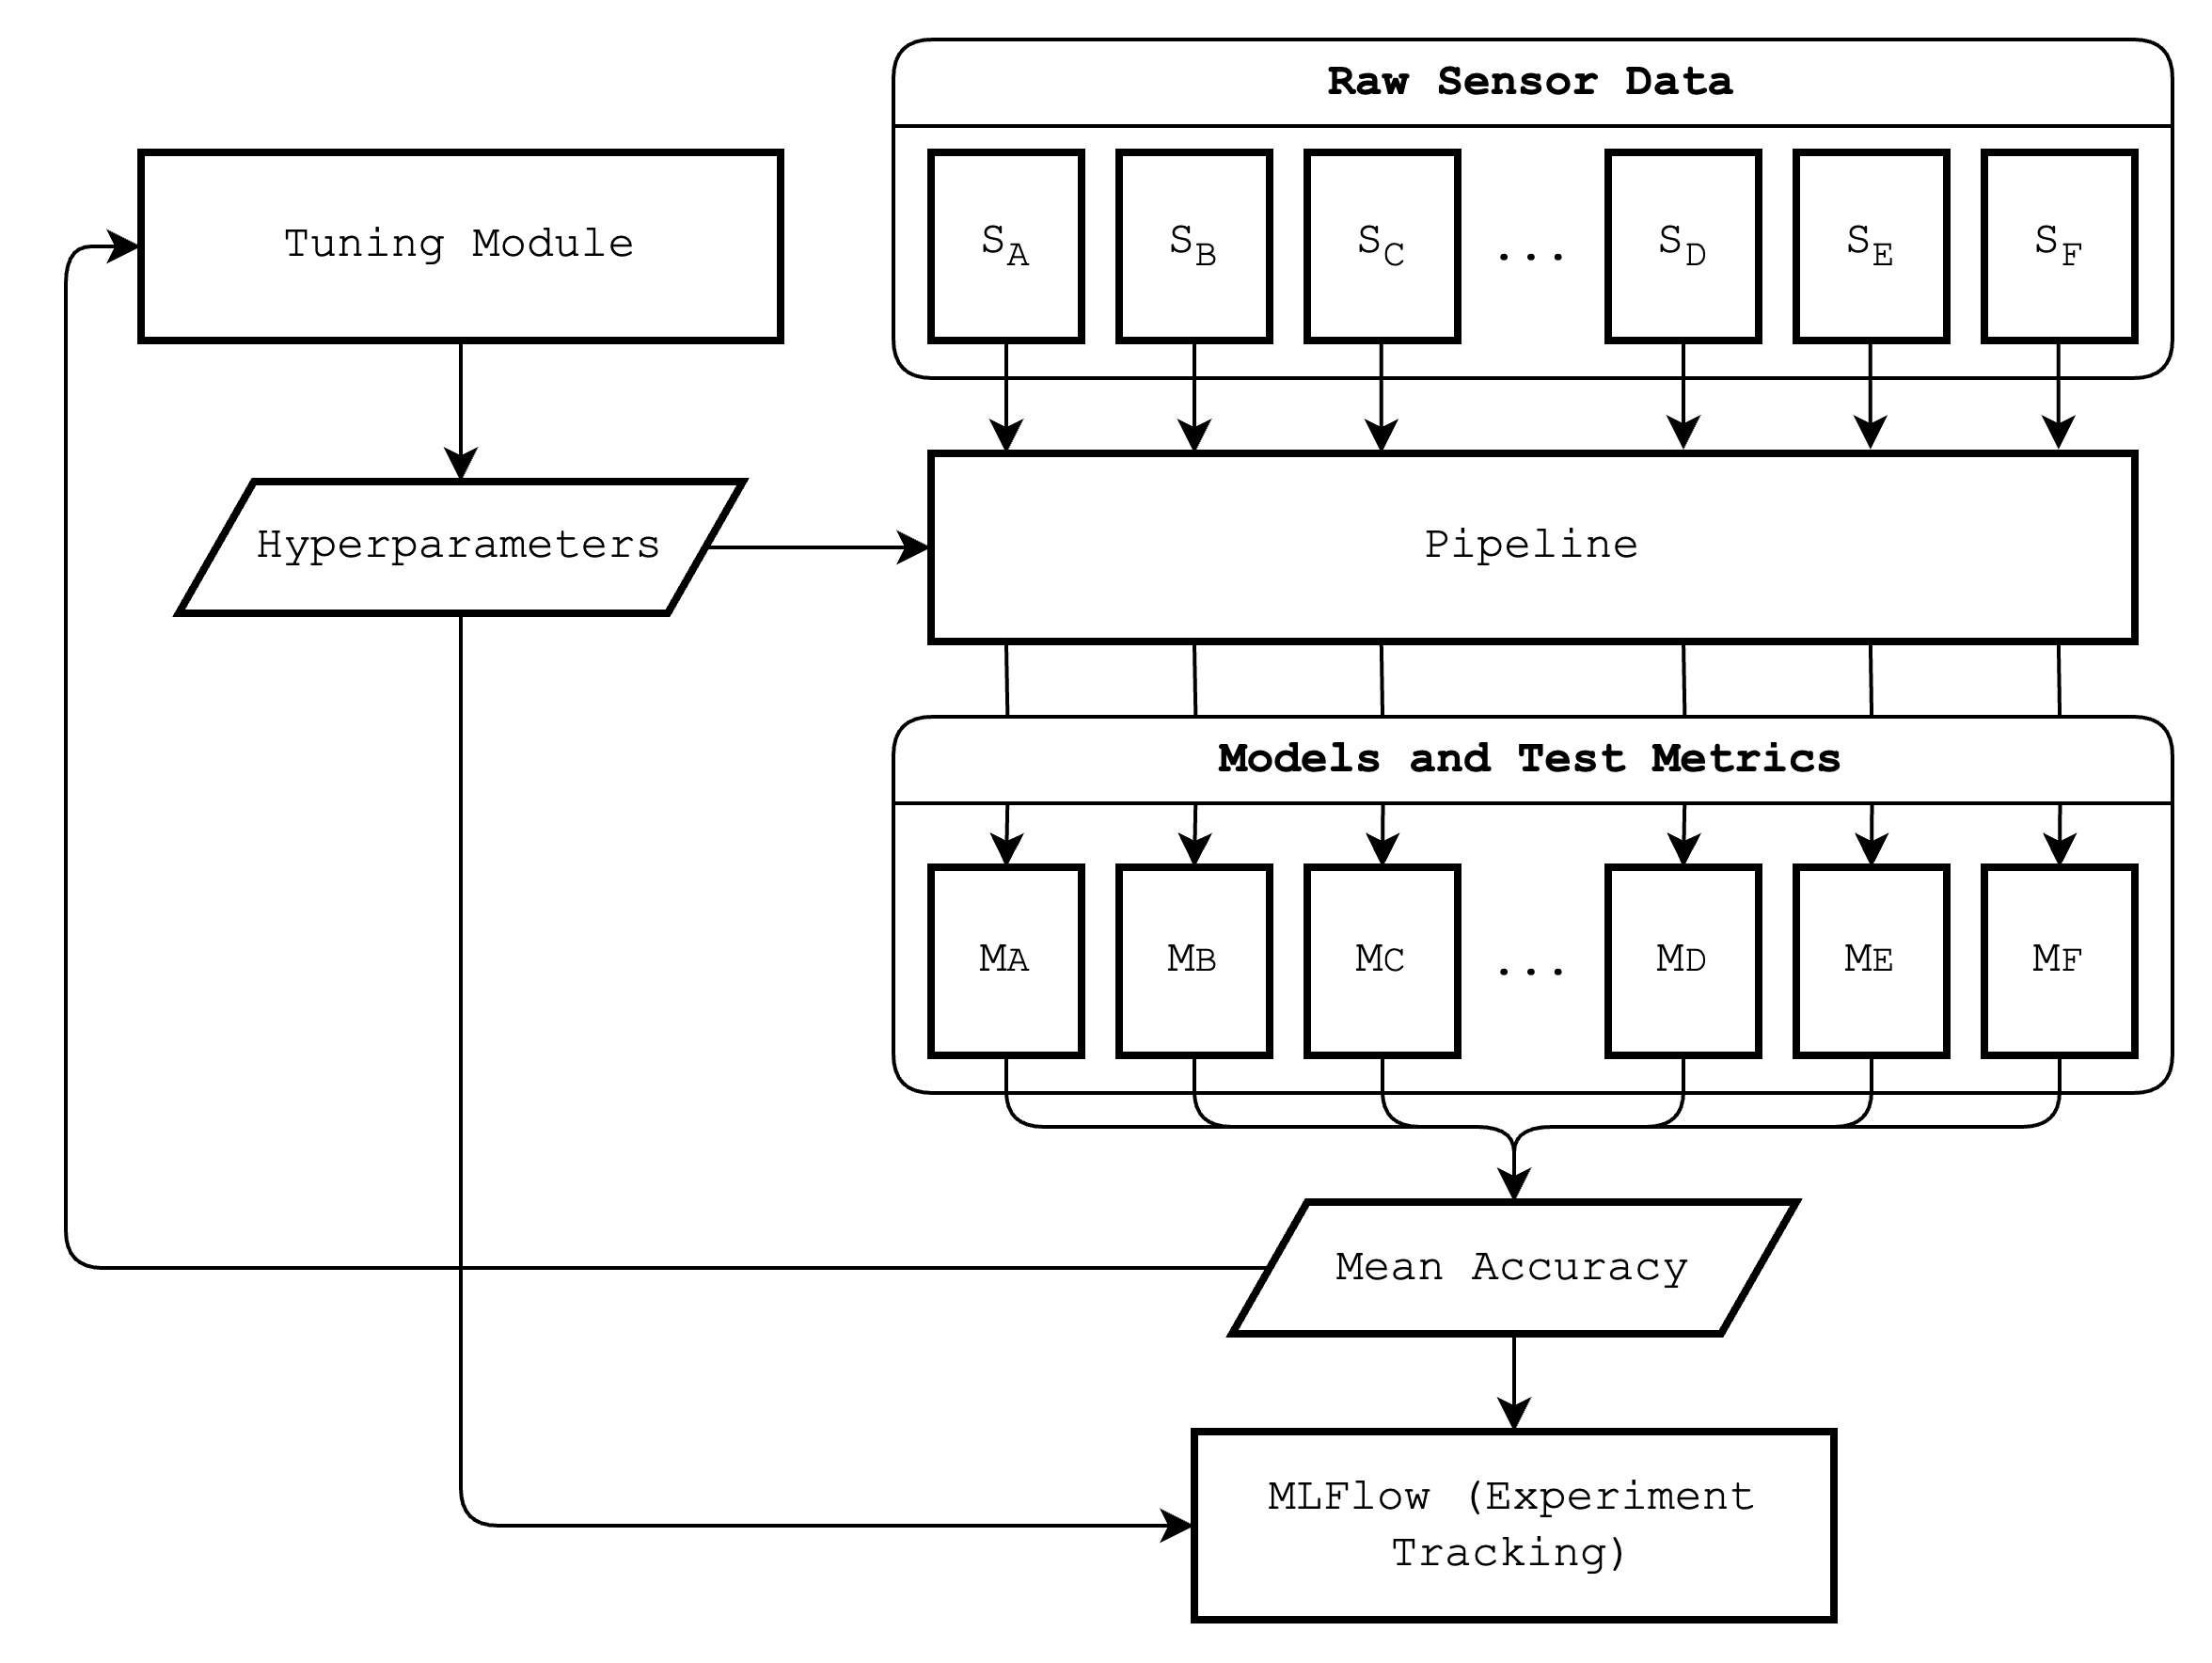
\includegraphics[width=\textwidth]{figures/methodology/hyperparameter_tuning.png}
    \caption{Hyper-parameter tuning process}
    \label{fig:hyperparameter_tuning}
\end{figure}

\subsubsection{Real-Time Monitoring System}
\begin{itemize}
    \item System architecture - how is this designed - open source - reproducible - executable?
    \item Event detection  - how is this implemented?
    \item Dashboard development - what is the purpose and use of the dashboard?
\end{itemize}

\subsubsection{Data Collection}

\begin{figure}[H]
    \centering
    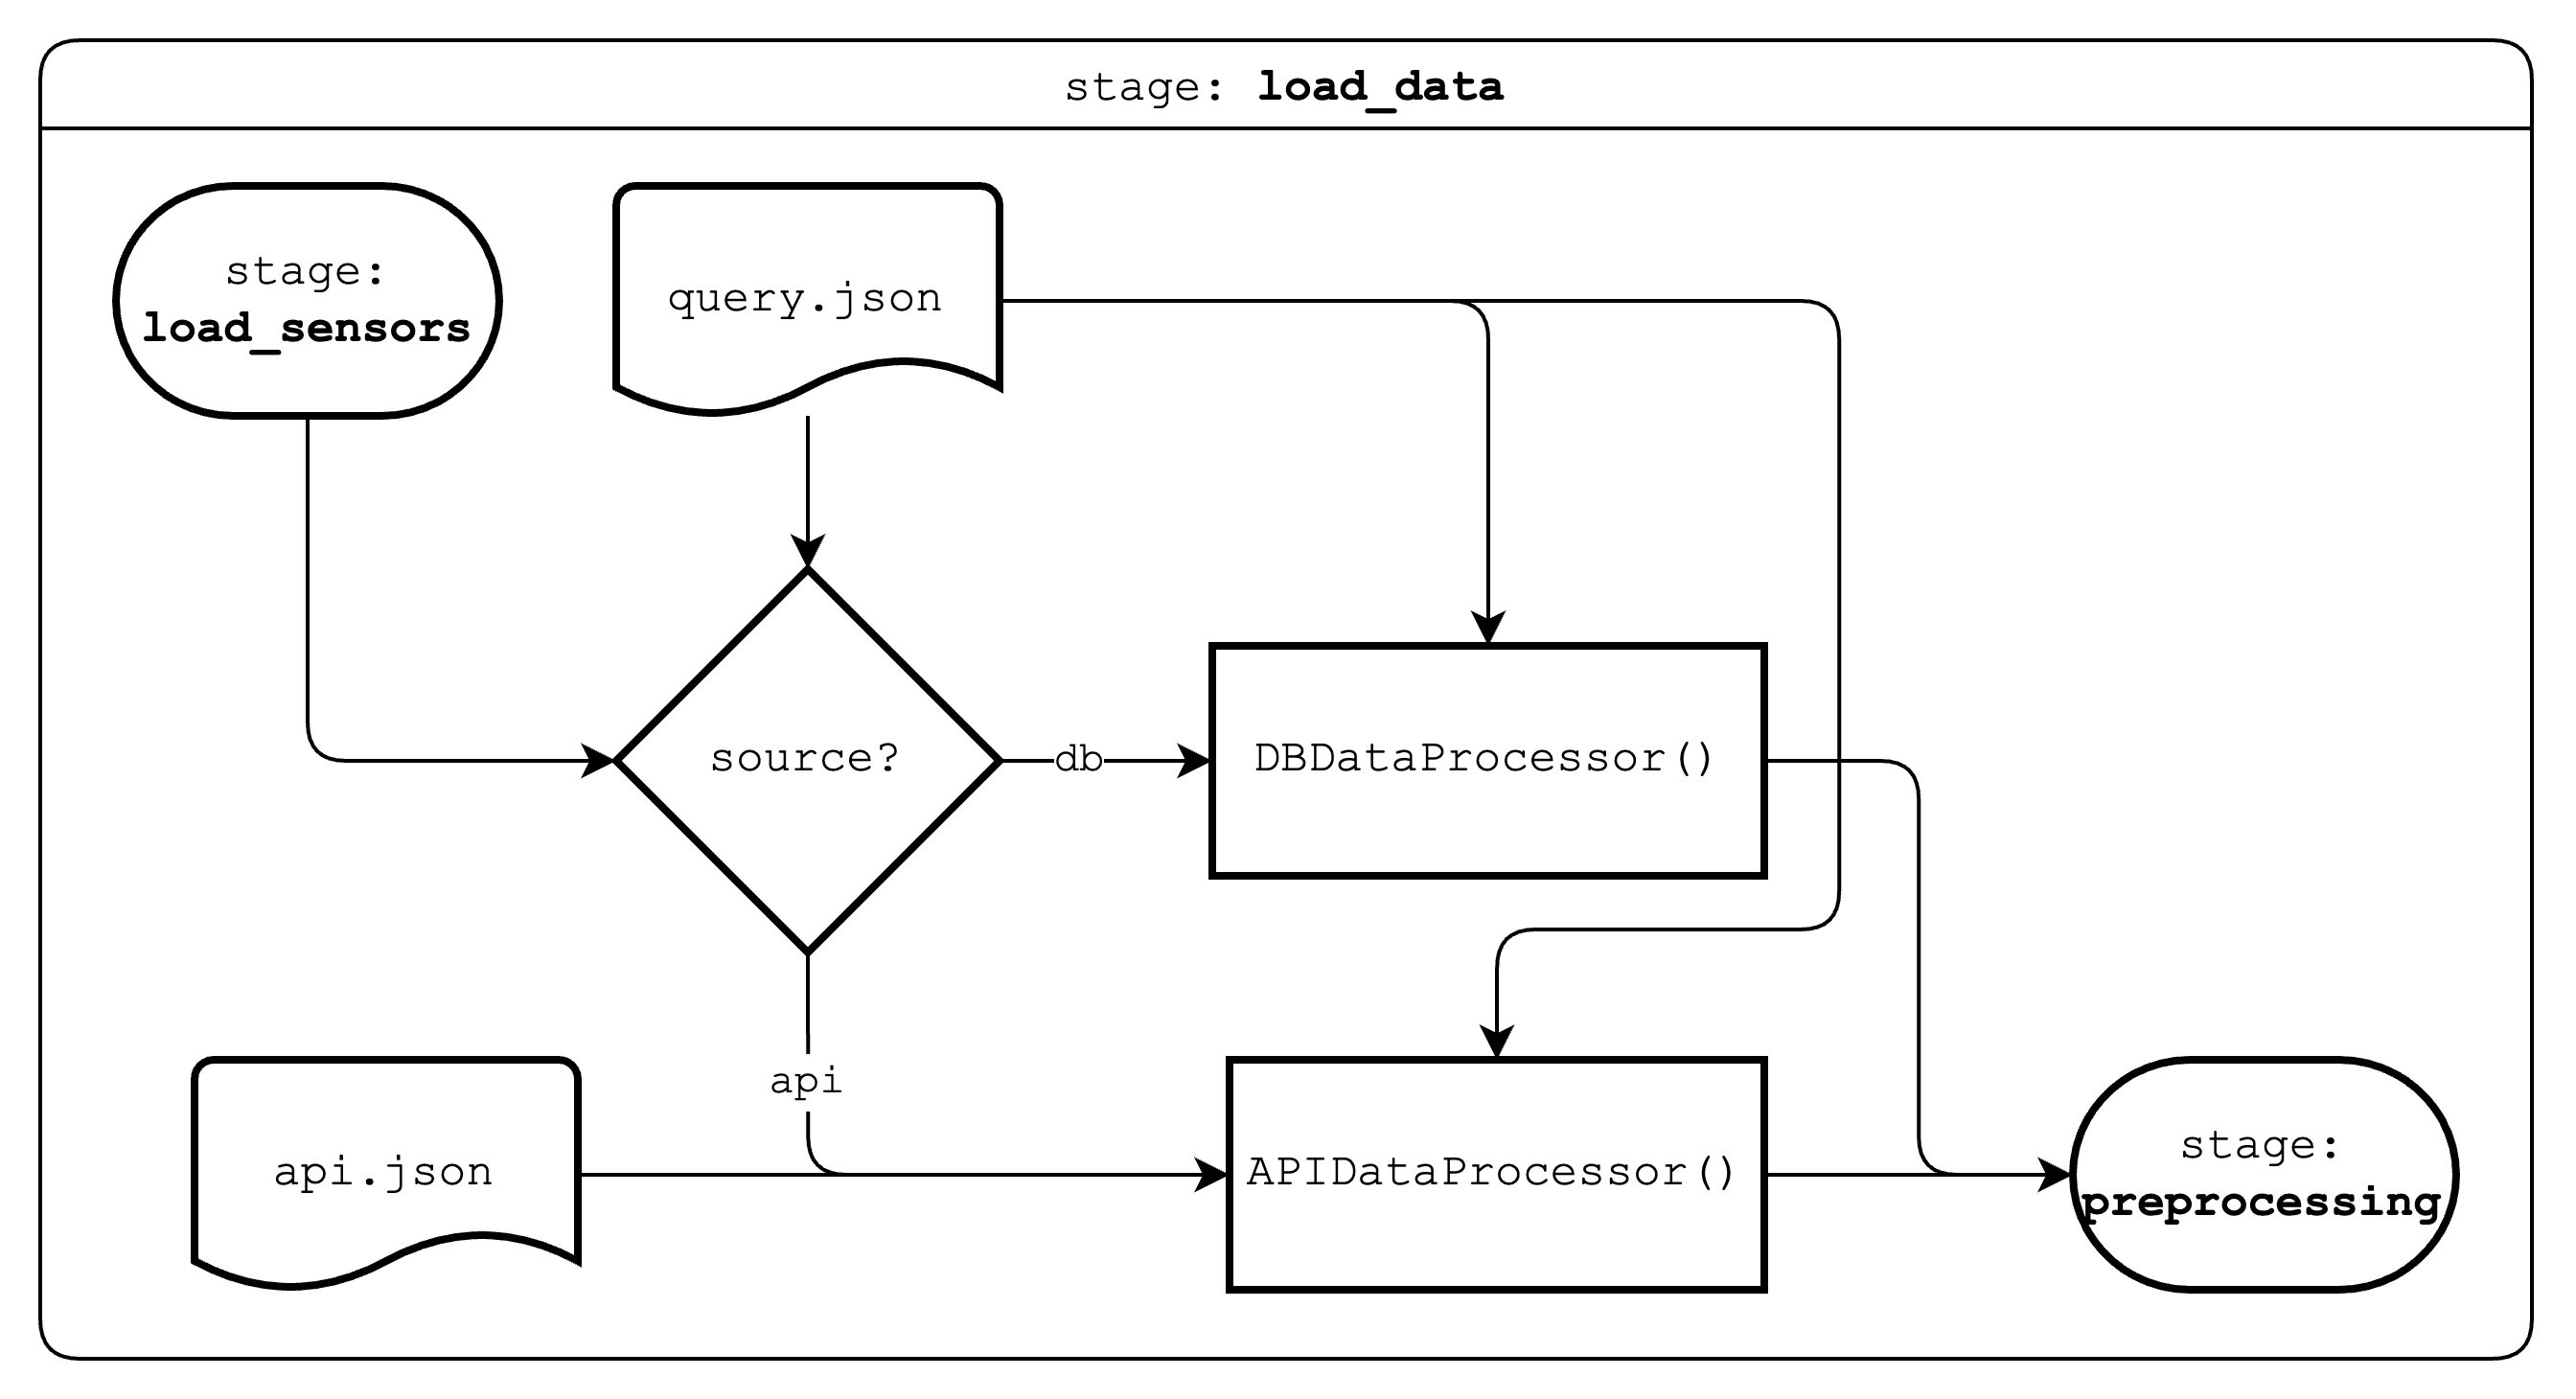
\includegraphics[width=\textwidth]{figures/methodology/load_data_stage.png}
    \caption{Loading data into the pipeline}
    \label{fig:load_data}
\end{figure}

\subsubsection{Data Preprocessing}
\label{subsubsection: imp_data_preprocessing}
(Diagram for Data Preprocessing)

\begin{figure}[H]
    \centering
    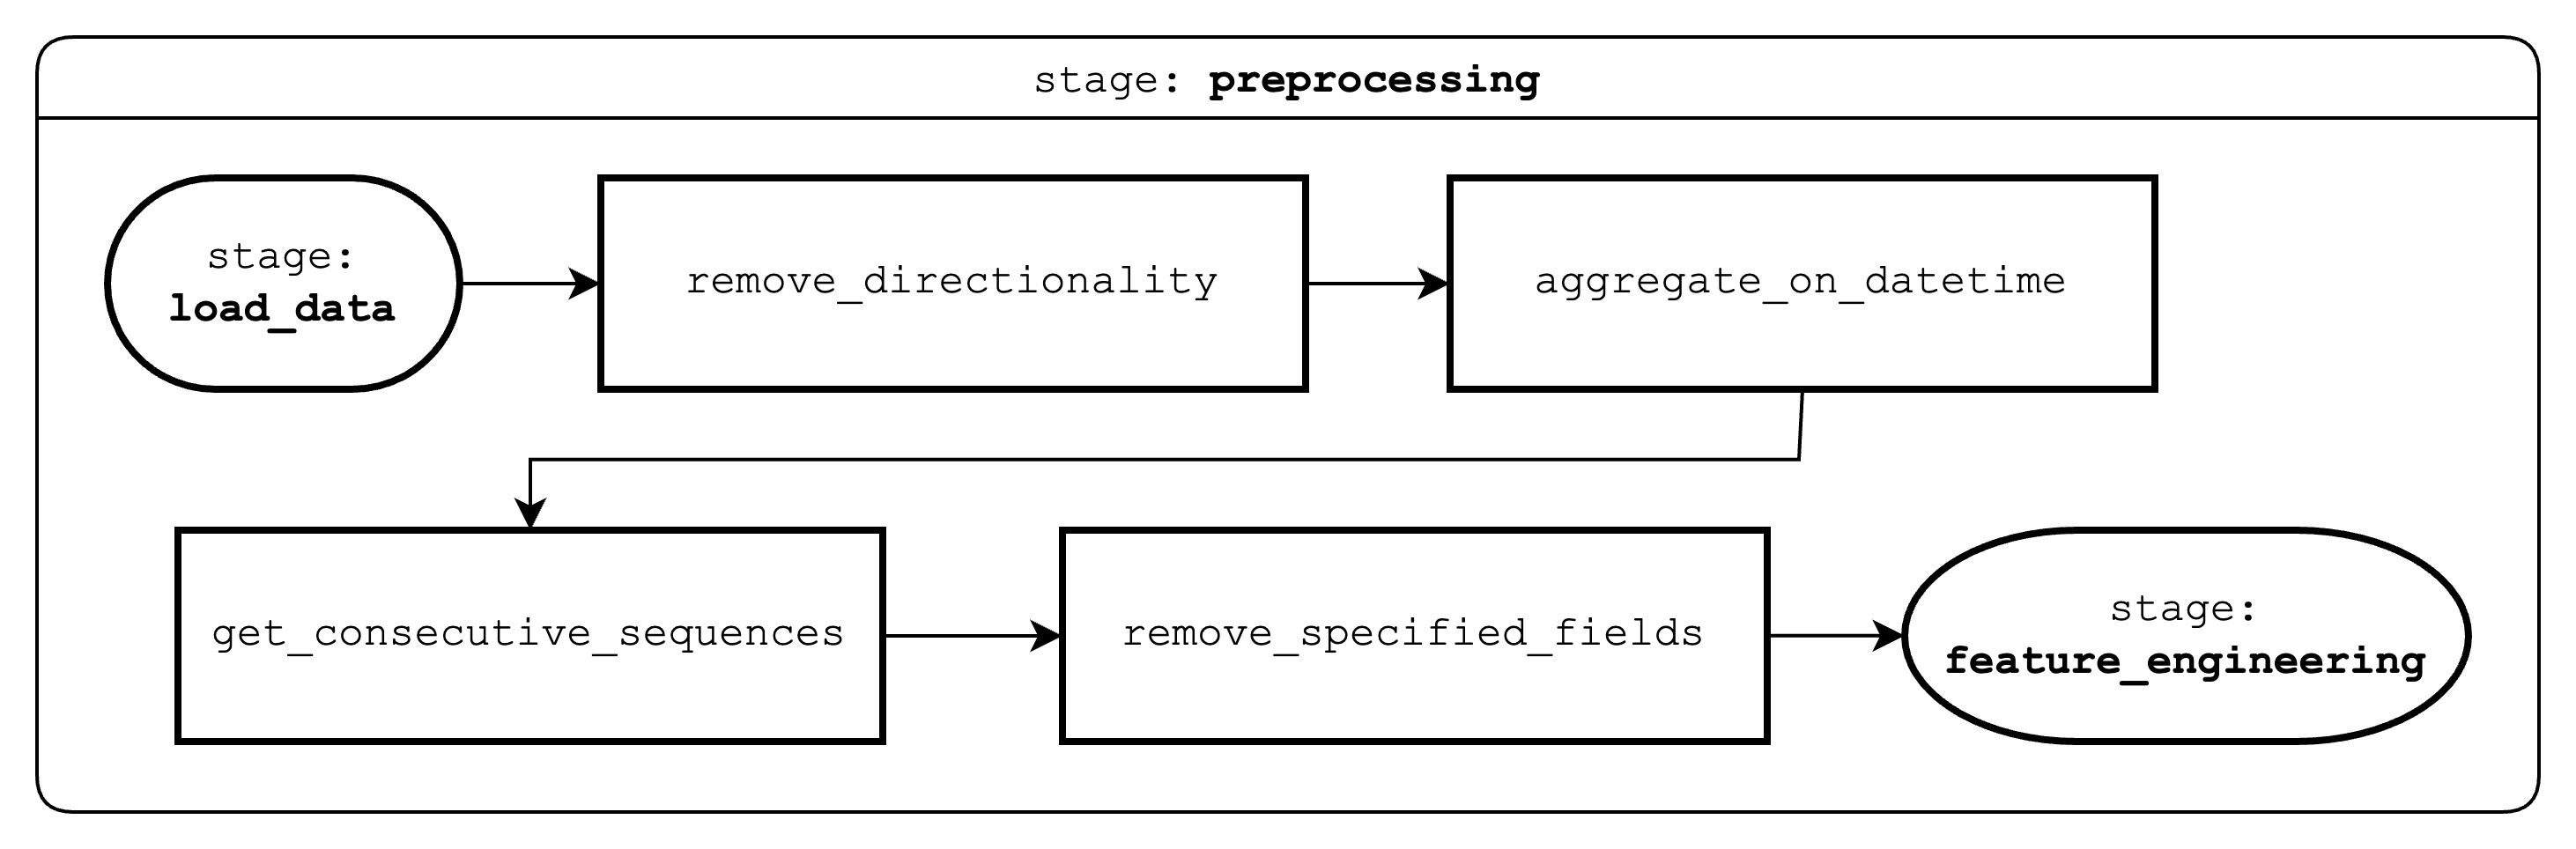
\includegraphics[width=\textwidth]{figures/methodology/preprocessing_stage.png}
    \caption{Data preprocessing stage}
    \label{fig:preprocessing}
\end{figure}

\begin{algorithm}
    \caption{Find and process consecutive sequences}
    \begin{algorithmic}[1]
        \Require DataFrame $df$ with time series data
        \Ensure DataFrame with consecutive sequences and assigned sequence numbers

        \Function{ProcessConsecutiveSequences}{$df$}
        \State $sequences \gets \emptyset$
        \State $current\_sequence \gets \emptyset$
        \State $\Delta t_{min} \gets$ minimum time delta between timestamps
        \State $w \gets$ window size
        \State $h \gets$ horizon

        \For{each row $r$ in $df$}
        \If{$current\_sequence = \emptyset$ \textbf{or} time difference between $r$ and last row of $current\_sequence = \Delta t_{min}$}
        \State Add $r$ to $current\_sequence$
        \Else
        \If{length of $current\_sequence > w + h$}
        \State Add $current\_sequence$ to $sequences$
        \EndIf
        \State $current\_sequence \gets \{r\}$
        \EndIf
        \EndFor

        \If{length of $current\_sequence > w + h$}
        \State Add $current\_sequence$ to $sequences$
        \EndIf

        \State $result \gets \emptyset$
        \For{$i \gets 1$ to $|sequences|$}
        \State Assign sequence number $i$ to all rows in $sequences[i]$
        \State Add $sequences[i]$ to $result$
        \EndFor

        \State \Return $result$
        \EndFunction
    \end{algorithmic}
    \label{alg:process_consecutive_sequences}
\end{algorithm}[H]

\subsubsection{Feature Engineering}
(Diagram for Feature Engineering)

The algorithm runs in O(N) runtime which is optimal for this task as every element in the list needs to be inspected at least once.

\begin{figure}[H]
    \centering
    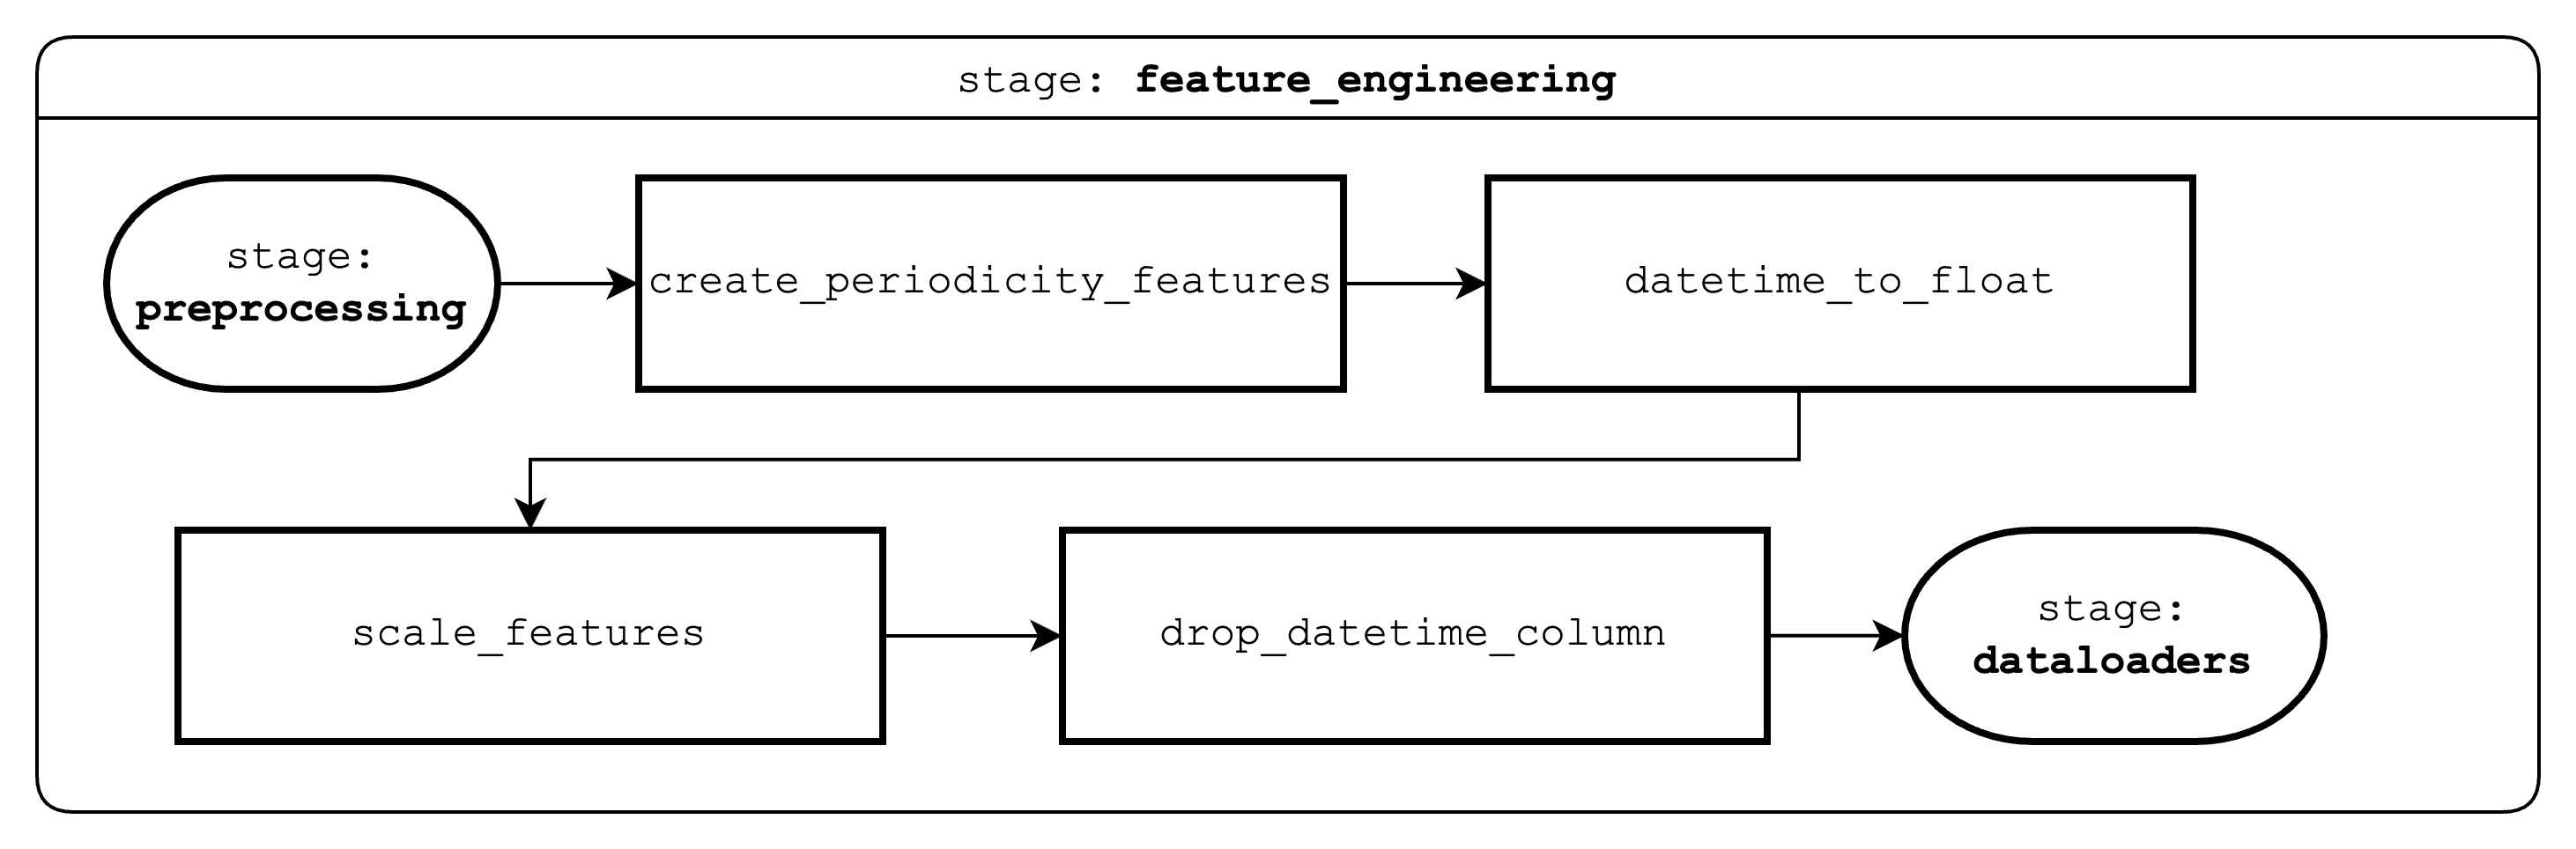
\includegraphics[width=\textwidth]{figures/methodology/feature_engineering_stage.png}
    \caption{Feature engineering stage}
    \label{fig:feature_engineering}
\end{figure}

\subsubsection{Machine Learning Pipeline Development}
(Diagram for Machine Learning Pipeline Development)

\subsubsection{Real-Time Monitoring System}
(Diagram for Real-Time Monitoring System)

\subsubsection{Validation and Testing}
(Diagram for Validation and Testing)

\subsubsection{MLOPs}
\begin{figure}[H]
    \centering
    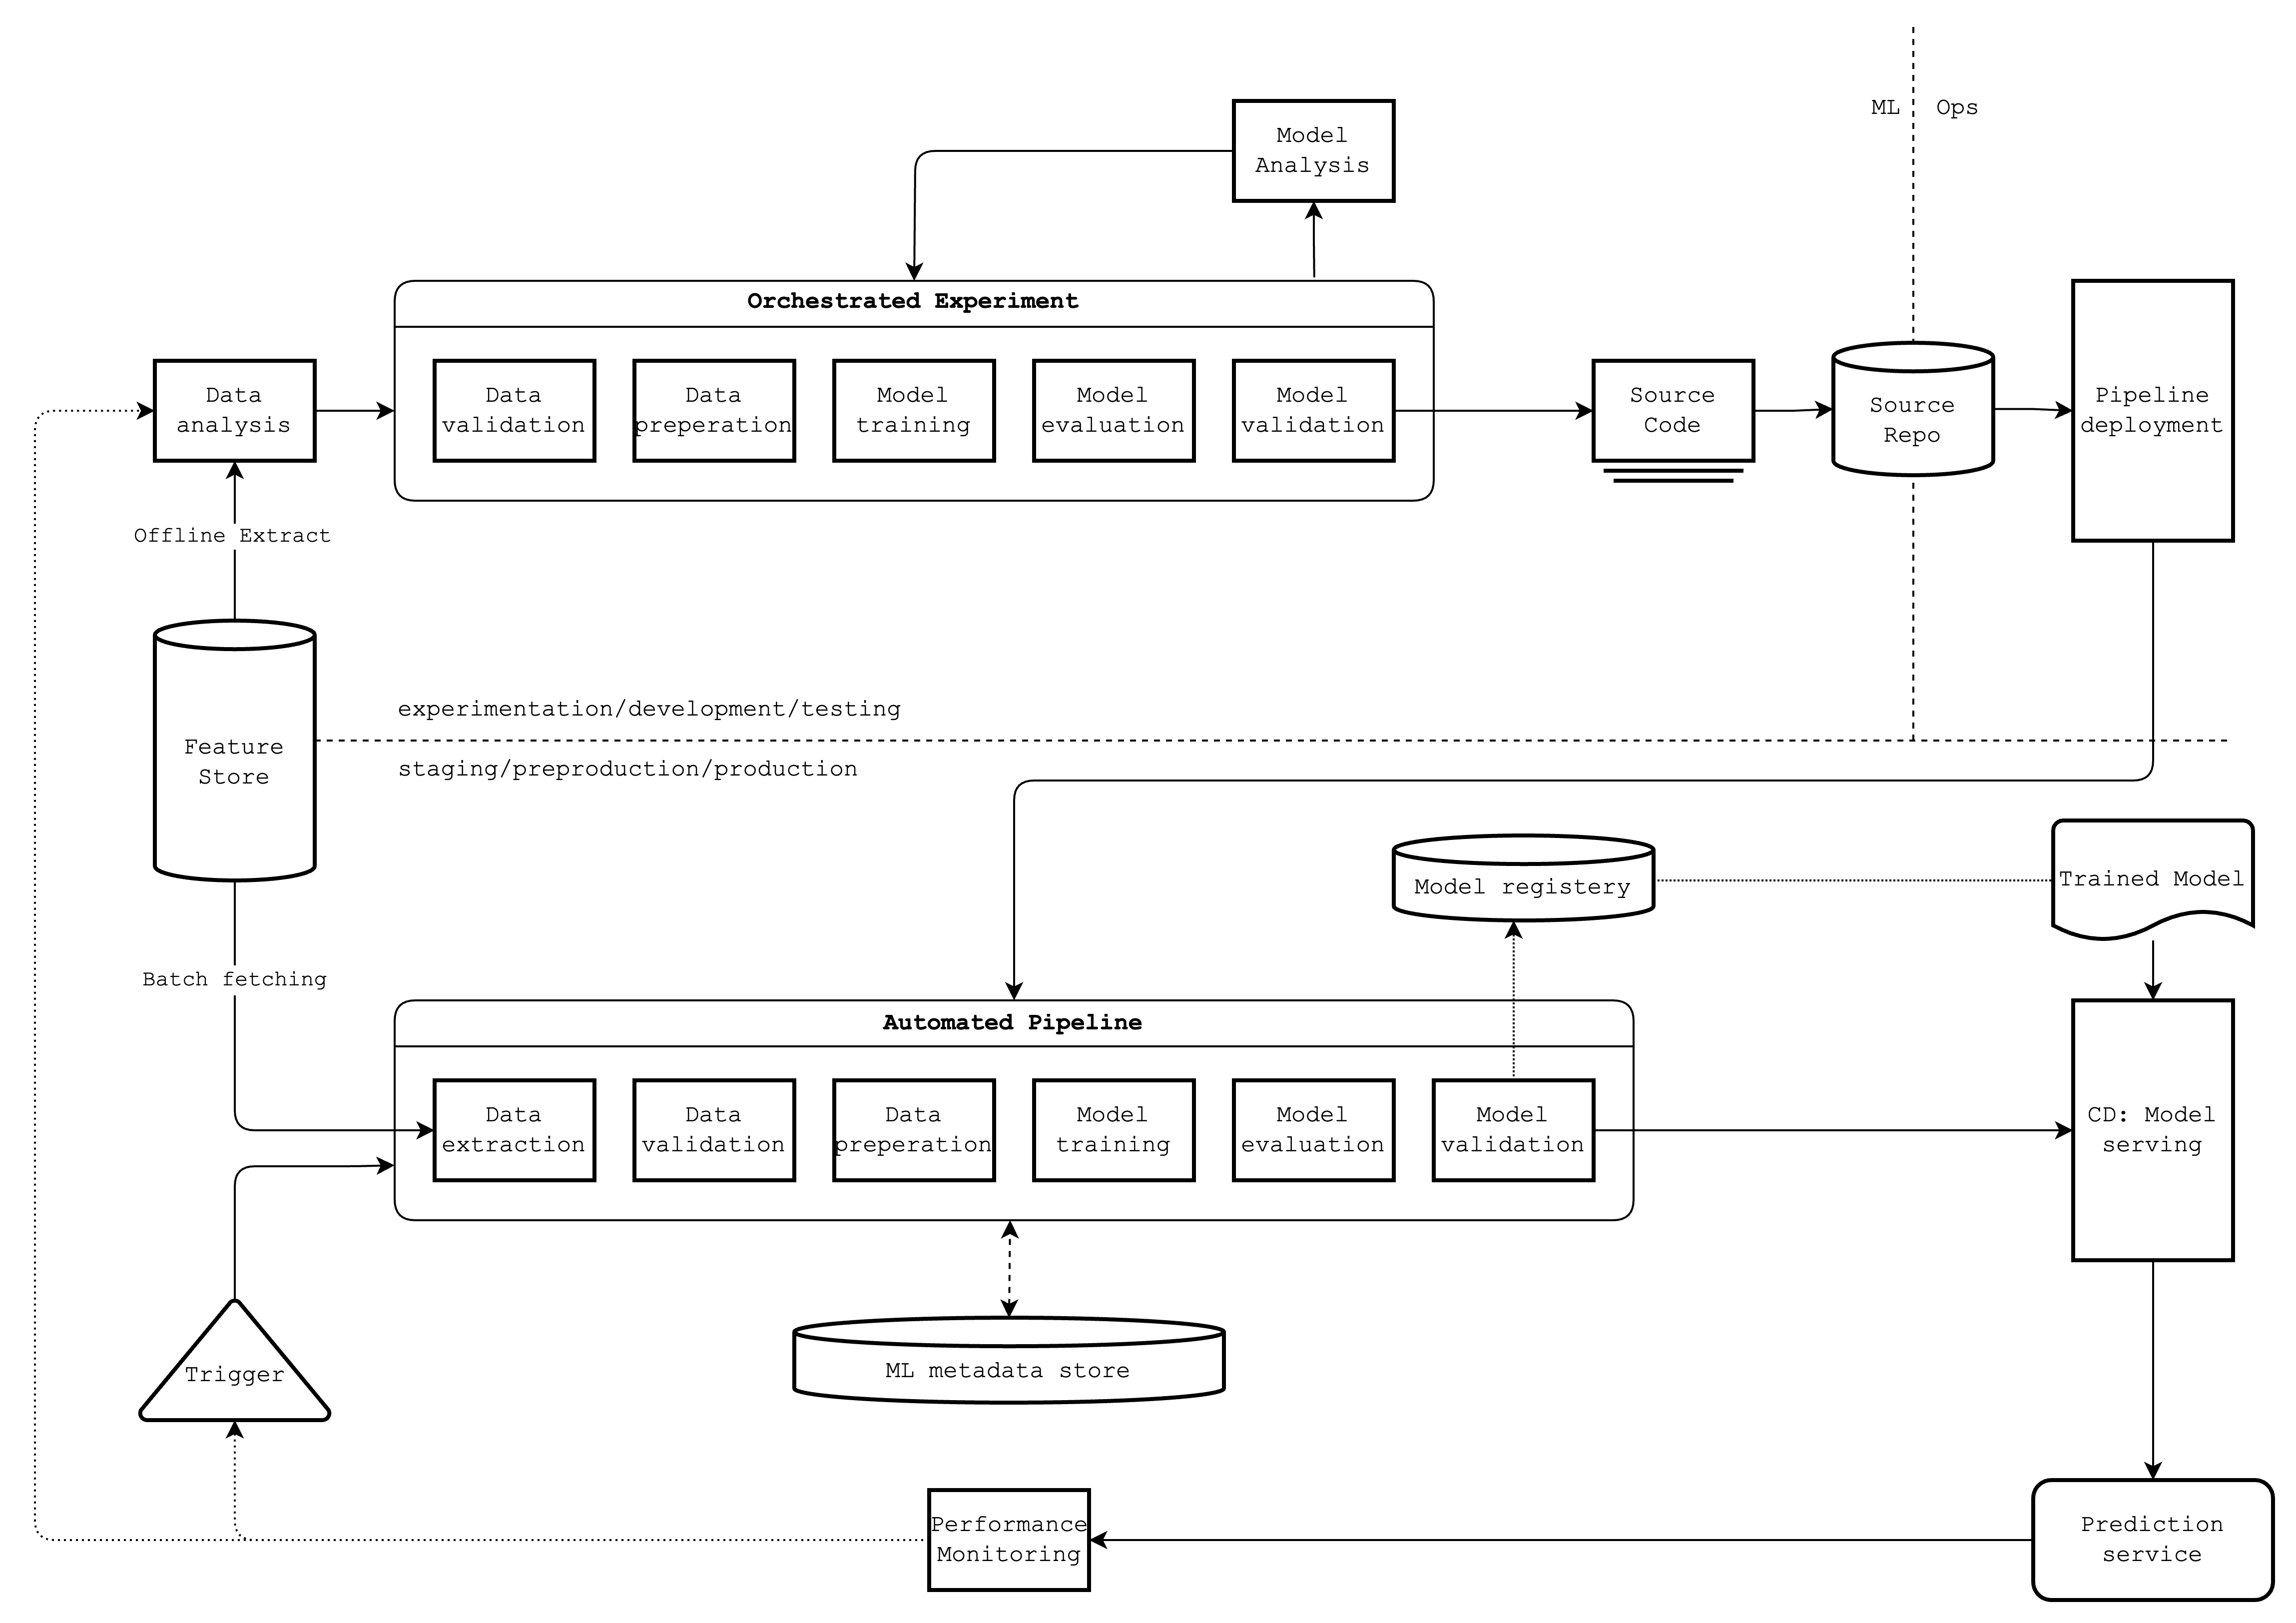
\includegraphics[width=\textwidth]{figures/methodology/mlops.png}
    \caption{MLOPs pipeline (based on \cite{kazmierczakMLOpsContinuousDelivery2024})}
    \label{fig:mlops}
\end{figure}

\subsubsection{Dashboard Development}
(Diagram for Dashboard Development)

For the development of the dashboard, a combination of Flask and Dash was chosen. This decision was based on several factors:

\begin{enumerate}
    \item Flask as the Web Framework: Flask is a lightweight, flexible, and extensible Python web framework. It provides a solid foundation for web applications without imposing a rigid structure, allowing for customisation and scalability.
    \item Dash for Interactive Visualisations: Dash, built on top of Flask, Plotly.js, and React.js, offers a powerful toolset for building analytical web applications. It provides a Python interface for creating reactive, web-based visualisations without the need for extensive JavaScript knowledge. This aligns well with the data-centric nature of this project and the preference for Python in the scientific community.
    \item Integration Capabilities: The combination of Flask and Dash allows for seamless integration with the existing Python-based machine learning pipeline. This integration ensures that real-time data from the sensors and outputs from the predictive models can be efficiently channeled into the dashboard.
    \item Customisability and Extensibility: Both Flask and Dash offer high levels of customisability. This is crucial for a research project where requirements may evolve, and new visualisations or features may need to be added as the project progresses.
    \item Performance: For real-time data visualisation, performance is critical. Both Flask and Dash are known for their efficiency in handling data streams and updating visualisations, making them suitable for monitoring live sensor data.
\end{enumerate}

The dashboard incorporates several key features designed to effectively communicate data quality issues:
\begin{enumerate}
    \item Real-time Data Visualisation: Live plots showing incoming sensor data, allowing for immediate detection of anomalies or data quality issues.
    \item Quality Dimension Indicators: Visual representations of the various data quality dimensions identified in the literature review, such as completeness, accuracy, and timeliness.
    \item Alert System: An alert mechanism to notify users of significant deviations in data quality or potential sensor malfunctions.
    \item Historical Data View: The ability to view historical data and trends, enabling users to contextualise current data quality issues.
    \item Sensor Network Overview: A map-based interface showing the geographical distribution of sensors and their current status.
          Predictive Analytics Display: Visualisation of the outputs from the machine learning models, including predictions and confidence intervals.
\end{enumerate}

How does the dashboard link back to the data quality dimensions defined in the literature review?

\subsection{Expected Outcomes}

What are the three or four key messages that I want to convey?
\begin{itemize}
    \item An understanding of the data quality issues in urban observatories
    \item A pathway for developing a machine learning pipeline for automated data quality monitoring in smart cities
\end{itemize}

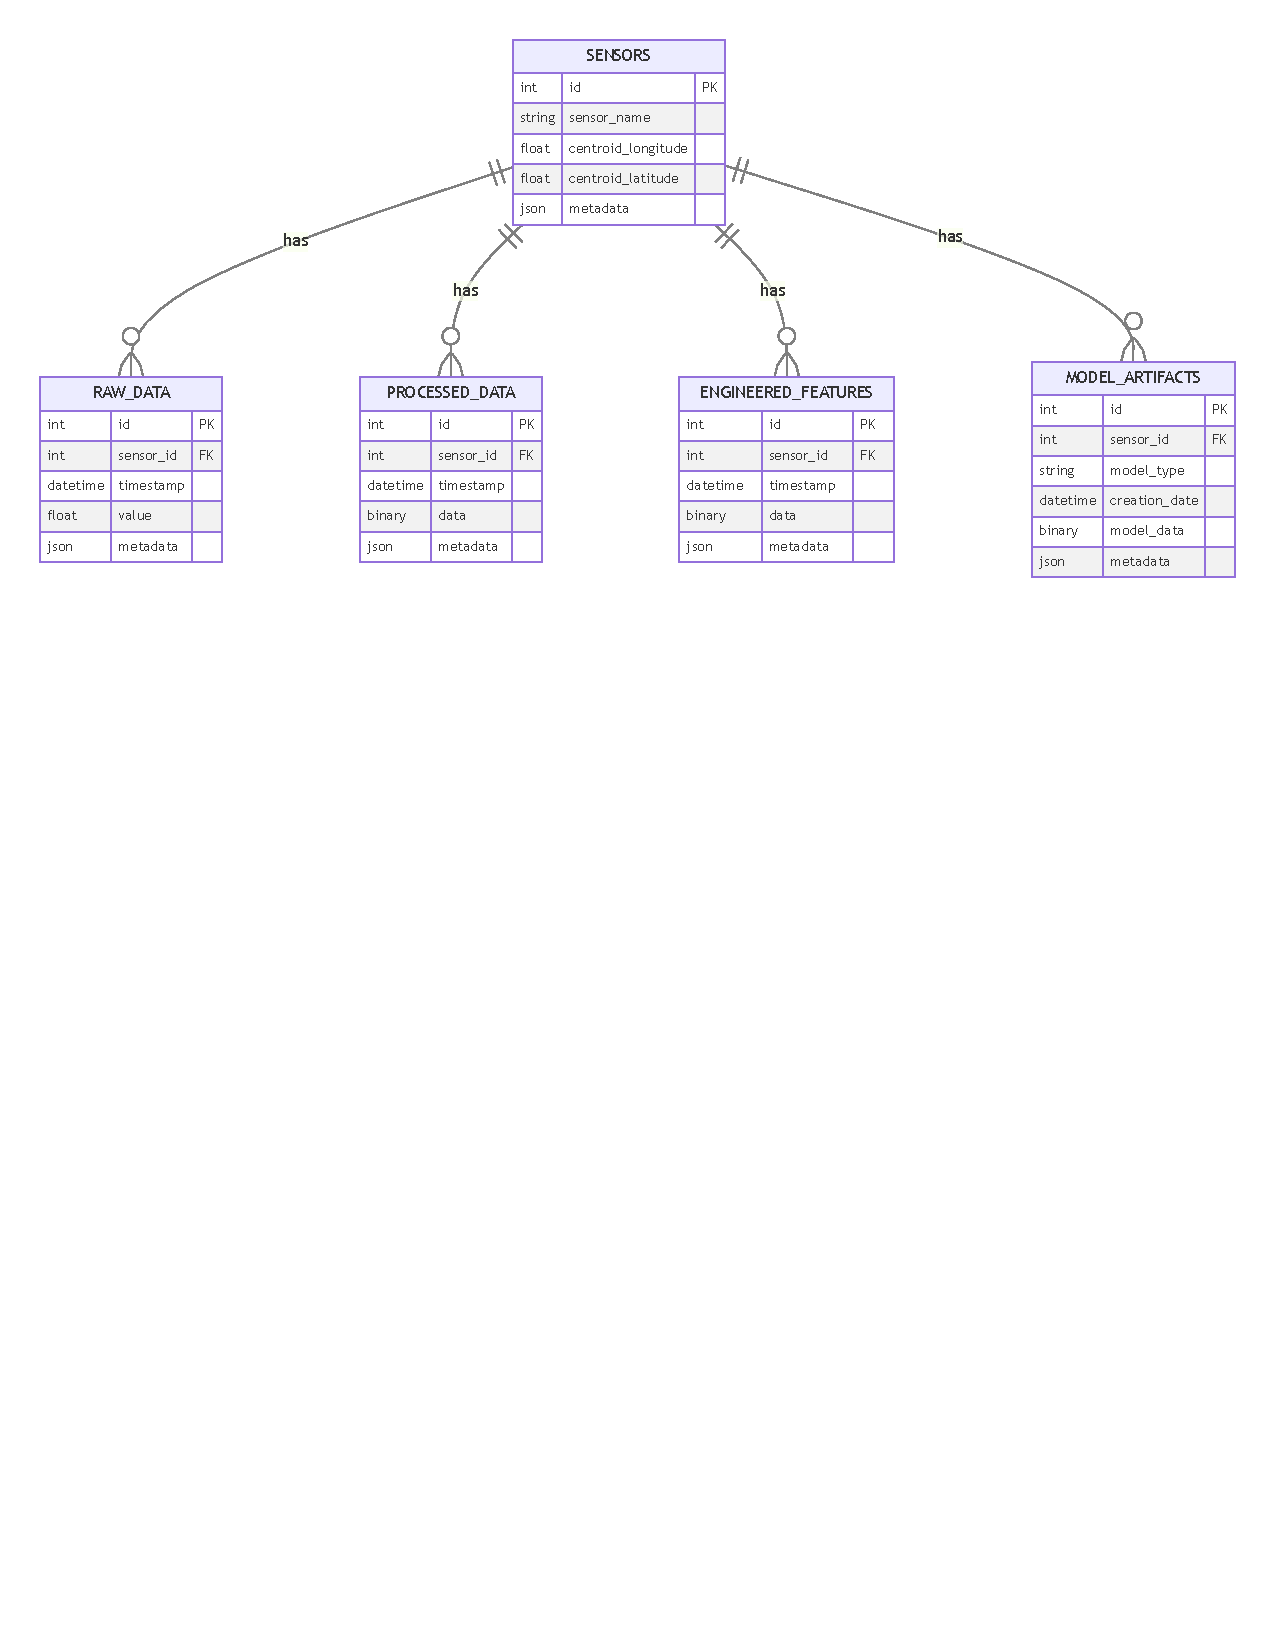
\includegraphics[width=\textwidth]{mermaid/database.pdf}
